%
%                  Politecnico di Milano
%
%         Student: Caravano Andrea, Alberto Cantele
%            A.Y.: 2024/2025
%
%   Last modified: 26/04/2025
%
%     Description: Internet of Things: Challenge n. 3
%                  Theoretical exercise
%

\documentclass[a4paper,11pt]{article} % tipo di documento
\usepackage[T1]{fontenc} % codifica dei font
\usepackage[utf8]{inputenc} % lettere accentate da tastiera
\usepackage[english]{babel} % lingua del documento
\usepackage{lipsum} % genera testo fittizio
\usepackage{url} % per scrivere gli indirizzi Internet e/o di riferimento nella pagina

\usepackage{hyperref} % per modificare il comportamento dei collegamenti ipertestuali

\usepackage[margin=0.7in]{geometry} % margine di pagina

\usepackage{graphicx} % per inserire immagini

\usepackage[outputdir=../auxil]{minted} % per colorazione automatica del codice (installare pygments da Homebrew)
% \usepackage{pythonhighlight} % per Python

\setminted{ % si può impostare il linguaggio specifico con \setminted[JSON] ad esempio
    linenos=true,
    breaklines=true,
    encoding=utf8,
    fontsize=\normalsize,
    frame=lines
}

\usepackage{fancyhdr}
\usepackage{textcomp}
\usepackage{siunitx} % per gestione intestazione e piè di pagina

\usepackage{tcolorbox} % per riquadrature di vario colore

\usepackage{float} % per figure comparative flottanti
\usepackage{amsmath} % per frazioni in display style

\usepackage{icomma} % virgola come separatore decimale

\usepackage{titlesec} % per configurazione del tipo paragrafo

\usepackage{multirow} % righe multiple in tabelle

\usepackage{subfig} % descrizione sottostante a figure

% setup del tipo paragrafo
\setcounter{secnumdepth}{4}

\titleformat{\paragraph}
{\normalfont\normalsize\bfseries}{\theparagraph}{1em}{}
\titlespacing*{\paragraph}
{0pt}{3.25ex plus 1ex minus .2ex}{1.5ex plus .2ex}

\hypersetup{ % metadati di titolo e autore nel PDF
    hidelinks, % leva colore attorno collegamenti ipertestuali
    pdftitle={Internet of Things: Challenge n. 3},
    pdfauthor={Andrea Caravano, Alberto Cantele}
}

\setlength{\parindent}{0pt} % rimuove l'indentazione del testo

\tcbset{ % impostazioni per riquadrature
    colback=gray!20,
    colframe=black,
    boxrule=0.5pt
}

\captionsetup{labelformat=empty} % rimuove la caption delle figure

% Imposta la profondità dell'indice a 2 livelli (sottosezioni, non sotto-sottosezioni)
\setcounter{tocdepth}{2}

\pagestyle{fancy}
\fancyhead{}\fancyfoot{}
\fancyhead[L]{\textbf{Internet of Things: Challenge n. 3}}
\fancyhead[R]{Andrea Caravano, Alberto Cantele}
\fancyfoot[C]{\thepage}

\title{\textbf{Internet of Things}\\Challenge n. 3: Theoretical exercise}
\author{Andrea Caravano, Alberto Cantele}
\date{Academic Year 2024--25}

\begin{document}
    \maketitle

    \tableofcontents


    \section{Question n. 1}\label{sec:question-n.-1}

    \subsection{Exercise text}\label{subsec:exercise-text}
    A LoRaWAN network in Europe (carrier frequency 868 MHz, bandwidth 125 kHz) is composed by one gateway and 50 sensor nodes.

    The sensor nodes transmit packet with payload size of L byte according to a Poisson process with intensity $\lambda$ = 1 packet / minute.

    Find the biggest LoRa SF for having a success rate of at least 70\%.

    For the payload size L of your packet, take it as follows:

    Take XY = Last two digit of your person code (leader code)

    $L = 3 + XY$ bytes

    \subsection{Problem analysis and preliminary computations}\label{subsec:problem-analysis-and-preliminary-computations}
    Let's approach the problem by delineating the known network parameters and identifying where we are aiming and therefore the missing pieces to complete the whole picture.

    \bigskip

    Given

    \medskip

    $N = 50$ sensor nodes

    \smallskip

    $\lambda = 1$ packet/minute $= \dfrac{1}{60}$ packet/second

    \medskip

    $L = 3 + XY = 3 + 60 = 63$ bytes

    \medskip

    We are aiming at computing the Aloha success rate, as seen during the course lectures:

    \bigskip

    Success Rate (SR) $= \dfrac{S}{G} = e^{-2G} = e^{-2N\lambda t}$

    \bigskip

    Where we are clearly missing $t$, the airtime of the packet.

    \subsection{The Airtime Calculator and boundaries in calculations}\label{subsec:the-airtime-calculator-and-boundaries-in-calculations}

    \textsc{The Things Network}, an open-source infrastructure aiming at providing networking coverage for \textsc{LoRaWAN} made available a calculator tool, returning the packet's airtime when given with the required problem data.

    \smallskip

    In particular, the following problem data are used:

    \medskip

    \begin{tabular}{|c|c|}
        \hline
        Parameter        & Value        \\
        \hline
        L                & 63 bytes     \\
        \hline
        Spreading Factor & SF7-SF9      \\
        \hline
        Region           & EU (868 MHz) \\
        \hline
        Bandwidth        & 125 kHz      \\
        \hline
    \end{tabular}

    \bigskip

    Returning:

    \medskip

    \begin{tabular}{|c|c|c|c|c|}
        \hline
        L                   & Spreading Factor (SF) & Region                        & Bandwidth                & Resulting airtime \\
        \hline
        \multirow{3}{*}{63} & SF7                   & \multirow{3}{*}{EU (868 MHz)} & \multirow{3}{*}{125 kHz} & 138,5 ms          \\
        \cline{2-2} \cline{5-5}
        & SF8                   &                               &                          & 246,3 ms          \\
        \cline{2-2} \cline{5-5}
        & SF9                   &                               &                          & 451,6 ms          \\
        \hline
    \end{tabular}

    \bigskip

    \label{limit-sf}

    The airtime calculator, however, reminds us of the limitations imposed to higher Spreading Factors, limiting the maximum size of the packet length to $L = 51$ bytes.

    \smallskip

    The following computations, therefore, are required to put an artificial limit to the payload size, as per requirements.

    \smallskip

    The provided problem data are now:

    \medskip

    \begin{tabular}{|c|c|}
        \hline
        Parameter        & Value        \\
        \hline
        L                & 51 bytes     \\
        \hline
        Spreading Factor & SF10-SF12    \\
        \hline
        Region           & EU (868 MHz) \\
        \hline
        Bandwidth        & 125 kHz      \\
        \hline
    \end{tabular}

    \bigskip

    Resulting in:

    \medskip

    \begin{tabular}{|c|c|c|c|c|}
        \hline
        L                   & Spreading Factor (SF) & Region                        & Bandwidth                & Resulting airtime \\
        \hline
        \multirow{3}{*}{51} & SF10                  & \multirow{3}{*}{EU (868 MHz)} & \multirow{3}{*}{125 kHz} & 698,4 ms          \\
        \cline{2-2} \cline{5-5}
        & SF11                  &                               &                          & 1560,6 ms         \\
        \cline{2-2} \cline{5-5}
        & SF12                  &                               &                          & 2793,5 ms         \\
        \hline
    \end{tabular}

    \subsection{Resolution}\label{subsec:resolution}
    We are now able to compute the Success Rate for all the problem configurations.

    \medskip

    Success Rate (SR) $= \dfrac{S}{G} = e^{-2G} = e^{-2N\lambda t}$

    \medskip

    Being the packet length and the Spreading Factors (on the spectrum) the only variable parameter among all configurations, they are chosen as a complete discriminant.

    \bigskip

    \begin{tabular}{|c|c|c|}
        \hline
        L                                  & Spreading Factor (SF) & Computation                                                                                                                                 \\
        \hline
        \multirow{3}{*}{\vspace{-2.3cm}63} & SF7                   & \rule{0pt}{6ex} $SR_{1} = \dfrac{S}{G} = e^{-2G} = e^{-2N\lambda t} = e^{-2 \cdot 50 \cdot \dfrac{1}{60} \cdot 0,1385} = 0,7939 = 79,39\%$ \\[3ex]
        \cline{2-3}
        & SF8                   & \rule{0pt}{6ex} $SR_{2} = \dfrac{S}{G} = e^{-2G} = e^{-2N\lambda t} = e^{-2 \cdot 50 \cdot \dfrac{1}{60} \cdot 0,2463} = 0,6633 = 66,33 \%$ \\[3ex]
        \cline{2-3}
        & SF9                   & \rule{0pt}{6ex} $SR_{3} = \dfrac{S}{G} = e^{-2G} = e^{-2N\lambda t} = e^{-2 \cdot 50 \cdot \dfrac{1}{60} \cdot 0,4516} = 0,4711 = 47,11 \%$ \\[3ex]
        \hline
        \multirow{3}{*}{\vspace{-2.3cm}51} & SF10                  & \rule{0pt}{6ex} $SR_{4} = \dfrac{S}{G} = e^{-2G} = e^{-2N\lambda t} = e^{-2 \cdot 50 \cdot \dfrac{1}{60} \cdot 0,6984} = 0,3122 = 31,22 \%$ \\[3ex]
        \cline{2-3}
        & SF11                  & \rule{0pt}{6ex} $SR_{5} = \dfrac{S}{G} = e^{-2G} = e^{-2N\lambda t} = e^{-2 \cdot 50 \cdot \dfrac{1}{60} \cdot 1,5606} = 0,0742 = 7,42 \%$ \\[3ex]
        \cline{2-3}
        & SF12                  & \rule{0pt}{6ex} $SR_{6} = \dfrac{S}{G} = e^{-2G} = e^{-2N\lambda t} = e^{-2 \cdot 50 \cdot \dfrac{1}{60} \cdot 2,7935} = 0,0095 = 0,95 \%$ \\[3ex]
        \hline
    \end{tabular}

    \bigskip

    From which the requirement constraints (requiring $SR \geq 70\%$) clearly line out the first configuration being the only one compatible.

    \smallskip

    Moreover, we can also define an additional constraint on packet airtime, which is even more general and can be applied to any payload size, once the number of nodes is fixed.

    \smallskip

    $SR = \dfrac{S}{G} = e^{-2G} = e^{-2N\lambda t} \geq 0,7 \Rightarrow e^{-2\cdot 50 \cdot \dfrac{1}{60} \cdot t} \geq 0,7 \Rightarrow -2 \cdot 50 \cdot \dfrac{1}{60} \cdot t \cdot \ln(e) \geq \ln(0,7) \Rightarrow t \leq \dfrac{\ln(0,7)}{-2 \cdot 50 \cdot \dfrac{1}{60} \cdot 1}$

    \smallskip

    $\Rightarrow t \leq 0,214 \ seconds = 214,0\ ms$

    \smallskip

    From which we derive that our second configuration is, in fact, invalid.

    \subsection{Automation via code (Python)}\label{subsec:automation-via-code-(python)}

    \subsubsection{Problem and constants declaration}

    \begin{minted}{Python}
n_nodes = 50  # nodes
Lambda = 1 / 60  # 1 packet over 1 minute = 60 seconds
# Maximum Spreading Factor allowed for a length L = 60 + 3 = 63 bytes is SF9: limiting L to 51 bytes, being the allowed maximum
# (see https://www.thethingsnetwork.org/airtime-calculator)
spreading_factors = ["SF7", "SF8", "SF9", "SF10", "SF11", "SF12"]
# (from SF10, L = 51 bytes is used, see notes)
t_airtimes = [0.1385, 0.2463, 0.4516, 0.6984, 1.5606, 2.7935]  # seconds
    \end{minted}

    Where we identify the \hyperref[limit-sf]{limit imposed to higher Spreading Factor configurations}, as mentioned earlier.

    \subsubsection{Success Rate computation}

    \begin{minted}{Python}
# Success Rate computation is made using a loop to compute every computation with dfferent airtimes and a list to store the results
SR = []
for airtime in t_airtimes:
    SR.append(math.exp(-2 * n_nodes * Lambda * airtime))
    \end{minted}

    Where we automatically apply the Aloha Success Rate formula to all the configurations, \hyperref[subsec:resolution]{as mentioned}.

    \subsubsection{Determine the maximum Spreading Factor matching the constraints}

    \begin{minted}{Python}
# The maximum Spreading Factor matching the Success Rate constraints is determined through a trivial loop iterating on all Success Rate results computed earlier
# Among them, we are looking for the highest one still allowing a matching Success Rate (>= 0.7)
matching_SR = -1
while matching_SR + 1 < len(SR) and SR[matching_SR + 1] > 0.7:
    # Implicit assumption is that the minimum Spreading Factor matches the constraints
    matching_SR += 1

best_SF = spreading_factors[matching_SR]
print(
    f"The resulting maximum Spreading Factor with a Success Rate matching the constraints (>= 0.7) is: {best_SF}"
)
    \end{minted}

    Which results in the following output.

    \begin{tcolorbox}
        The resulting maximum Spreading Factor with a Success Rate matching the constraints (>= 0.7) is: SF7
    \end{tcolorbox}

    That confirms our theoretical expectations.


    \section{Question n. 2}\label{sec:question-n.-2}

    \subsection{Exercise text}\label{subsec:exercise-text2}

    You have purchased an Arduino MKR WAN 1310 and wish to create a system that reads temperature and humidity data from a DHT22 sensor and sends this data wirelessly to ThingSpeak over LoRaWAN.

    \smallskip

    Design a complete system block diagram (sketch in Node-Red) and describe, in detail, the steps you would need to take to get the system fully operational.

    \subsection{The Arduino MKR WAN 1310 board and the DHT-22 sensor}\label{subsec:the-arduino-mkr-wan-1310-board-and-the-dht-22-sensor}

    First, let's start by preparing our local environment, connecting the \textsc{Arduino} \textsc{LoRa}-enabled board to the \textsc{DHT-22} temperature and humidity sensor.

    \smallskip

    This translates to the following diagram.

    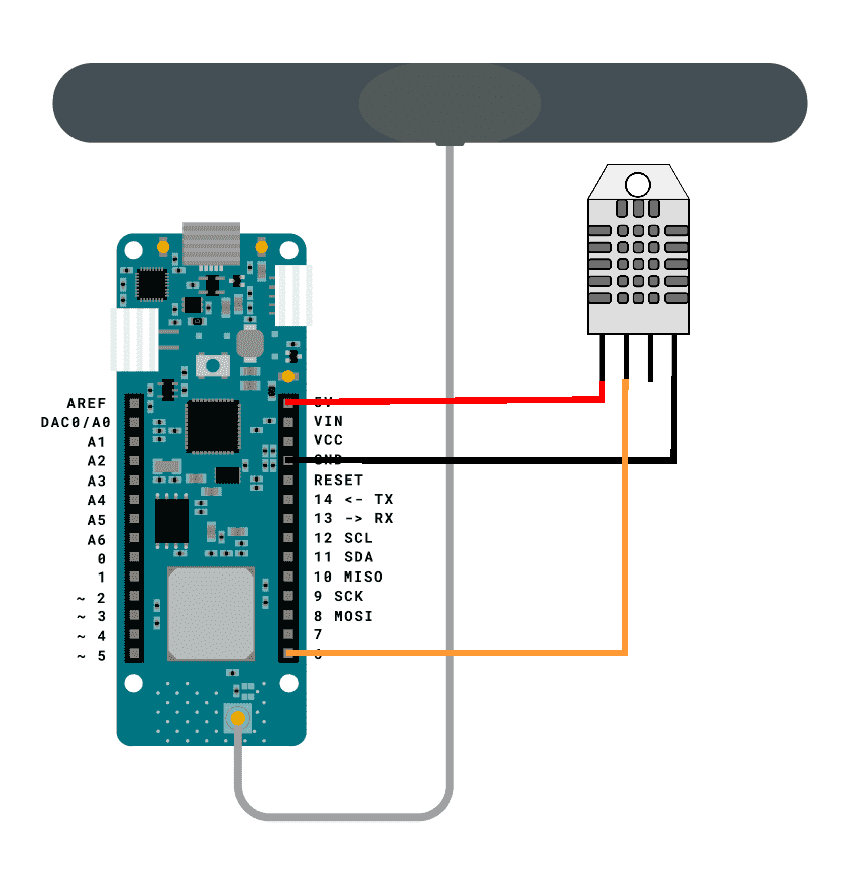
\includegraphics[width=10cm]{../res/arduino-dht22}

    Then, the \textsc{Arduino IDE} and related software should be installed and setup on the local development environment.

    \subsection{The Things Network}\label{subsec:the-things-network}

    \textsc{The Things Network} (TTN) is an open-source infrastructure (and network server, the most intelligent part of a LoRa network) aiming at providing free LoRaWAN network coverage.

    \smallskip

    The project is actively maintained by a growing community across the world, on a voluntary basis.

    \smallskip

    Gateways are incrementally being deployed across the globe, providing an increasing network coverage.

    \medskip

    \textsc{The Things Network} plays, more or less, the same role that a mobile radio network operator plays for mobile User Terminals: it provides the user with the connectivity and managerial services of their LoRaWAN provisions.

    \smallskip

    \subsubsection{Authentication in LoRa-based networks}

    Being the communication medium intrinsically shared among network nodes, authentication and security or \textsc{LoRa} communications play a fundamental role in its implementation.

    \smallskip

    The baseline encryption scheme is \textsc{AES-128}, implemented through a couple of keys: the \textsc{Network Session Key} for authentication and integrity and the \textsc{Application Session Key} for data encryption.

    \smallskip

    Two authentication/activation methods are supported:

    \begin{itemize}
        \item \textsc{Over-The-Air Activation (OOTA)}: The end-nodes are not initialized for any particular network: they will send a \textsc{JOIN Request} to a specific \textsc{LoRa}-based network (like \textsc{The Things Network}) and then receive a device address and an authorization token from which session keys are derived, starting from a root key pre-provisioned in the end-node by its manufacturer.

        This is the default and the preferred strategy.
        \item \textsc{Activation by Personalization (ABP)}: End devices are personalized to work with a specific \textsc{LoRa}-based network, right from its manufacturer.
        Session keys are pre-provisioned by the manufacturer, alongside the device network address.
    \end{itemize}

    \subsection{The Arduino board and The Things Network: integration overview}\label{subsec:the-arduino-board-and-the-things-network:integration-overview}

    \subsubsection{Register the board on the network}

    Before sending and receiving messages from \textsc{The Things Network}, the \textsc{Arduino} board must first be registered on the network.

    \smallskip

    For this, the board's \texttt{Device EUI} identifier must first be collected: the \textsc{MKRWAN} library embeds a specific function call (\texttt{modem.deviceEUI()}) that returns it.

    \medskip

    Once the \texttt{Device EUI} has been collected, a free account on \textsc{The Things Network} must be created.

    \smallskip

    Then, devices are expected to be registered with an application to communicate with: in the registration procedure, the \texttt{Device EUI} is asked, alongside some other security and identification parameters.

    \subsubsection{Connect the board to the network and send/receive packets}

    Once registered, the board can \textsc{Join} \textsc{The Things Network}.

    \smallskip

    A packet being sent is delineated by a \texttt{modem.beginPacket()} and a \texttt{modem.endPacket()} and sent through \texttt{modem.print()}, while a packet being received is read through \texttt{modem.read()}, after checking if available.

    \medskip

    In this step, some additional processing steps might be required to re-format the payload structure to adapt it to transmission rules.

    \medskip

    When considering further communication optimizations, one may consider the \hyperref[sec:question-n.-3]{characteristics lined out by Question n. 3, later}.

    \subsection{ThingSpeak}\label{subsec:thingspeak}

    \subsubsection{The Things Network integration}

    As mentioned during the course lectures, the Network Server (provided by \textsc{The Things Network}, in our case) is where most of the intelligence of the LoRa architecture is.

    \smallskip

    It also provides comfortable integrations for both MQTT and HTTP protocol stacks, related, in particular, to \textsc{ThingSpeak}, for which the default, however, is \textsc{HTTP}.

    \subsubsection{Collection of the measurements}

    The \textsc{DHT-22} temperature and humidity sensor is created defining a \texttt{DHT} object, clarifying the connection PIN and its model.

    \smallskip

    Subsequently, it is initialized in the \texttt{setup} phase through a \texttt{dht.begin()} function call.

    \medskip

    Then, temperature measurements are collected with \texttt{dht.readTemperature()} and humidity measurements with \texttt{dht.readHumidity()}.

    \smallskip

    Finally, the board packages sensor readings into a byte array and hands it off to the data preparation and transmission routines.

    \subsubsection{Channel creation}

    A \textsc{ThingSpeak} channel is a container for a variety of details related to a particular data collection and the data itself.

    \smallskip

    Being a \textsc{MATLAB} product, it also offers many possibilities for deeper data analysis.

    \smallskip

    Data streams are identified by \textsc{fields}, which are related to a single measurement: in our case, we will need to create two fields, for both temperature and humidity values.

    \smallskip

    Upon channel creation, the channel's ID and its write API key should be provided to \textsc{The Things Network}'s integration, as they will be used when forwarding data measurements gathered.

    \smallskip

    In this step, some additional processing steps might be required to re-format the payload structure to adapt it to the integration rules.

    \medskip

    By default, the chosen protocol is \textsc{HTTP}, through \textsc{POST} requests.

    \smallskip

    Note, however, that integrations using MQTT are also possible.

    \subsection{Node-RED sketched communication diagram}\label{subsec:node-red-sketched-communication-diagram}

    In the following, the \textsc{Inject} node represents the DHT-22 temperature and humidity sensor, while \textsc{The Things Network}'s network server and the \textsc{Arduino} board are simulated by a function node.

    \smallskip

    Finally, \textsc{LoRa}-specific uplink and downlink blocks close the communication loop.

    \medskip

    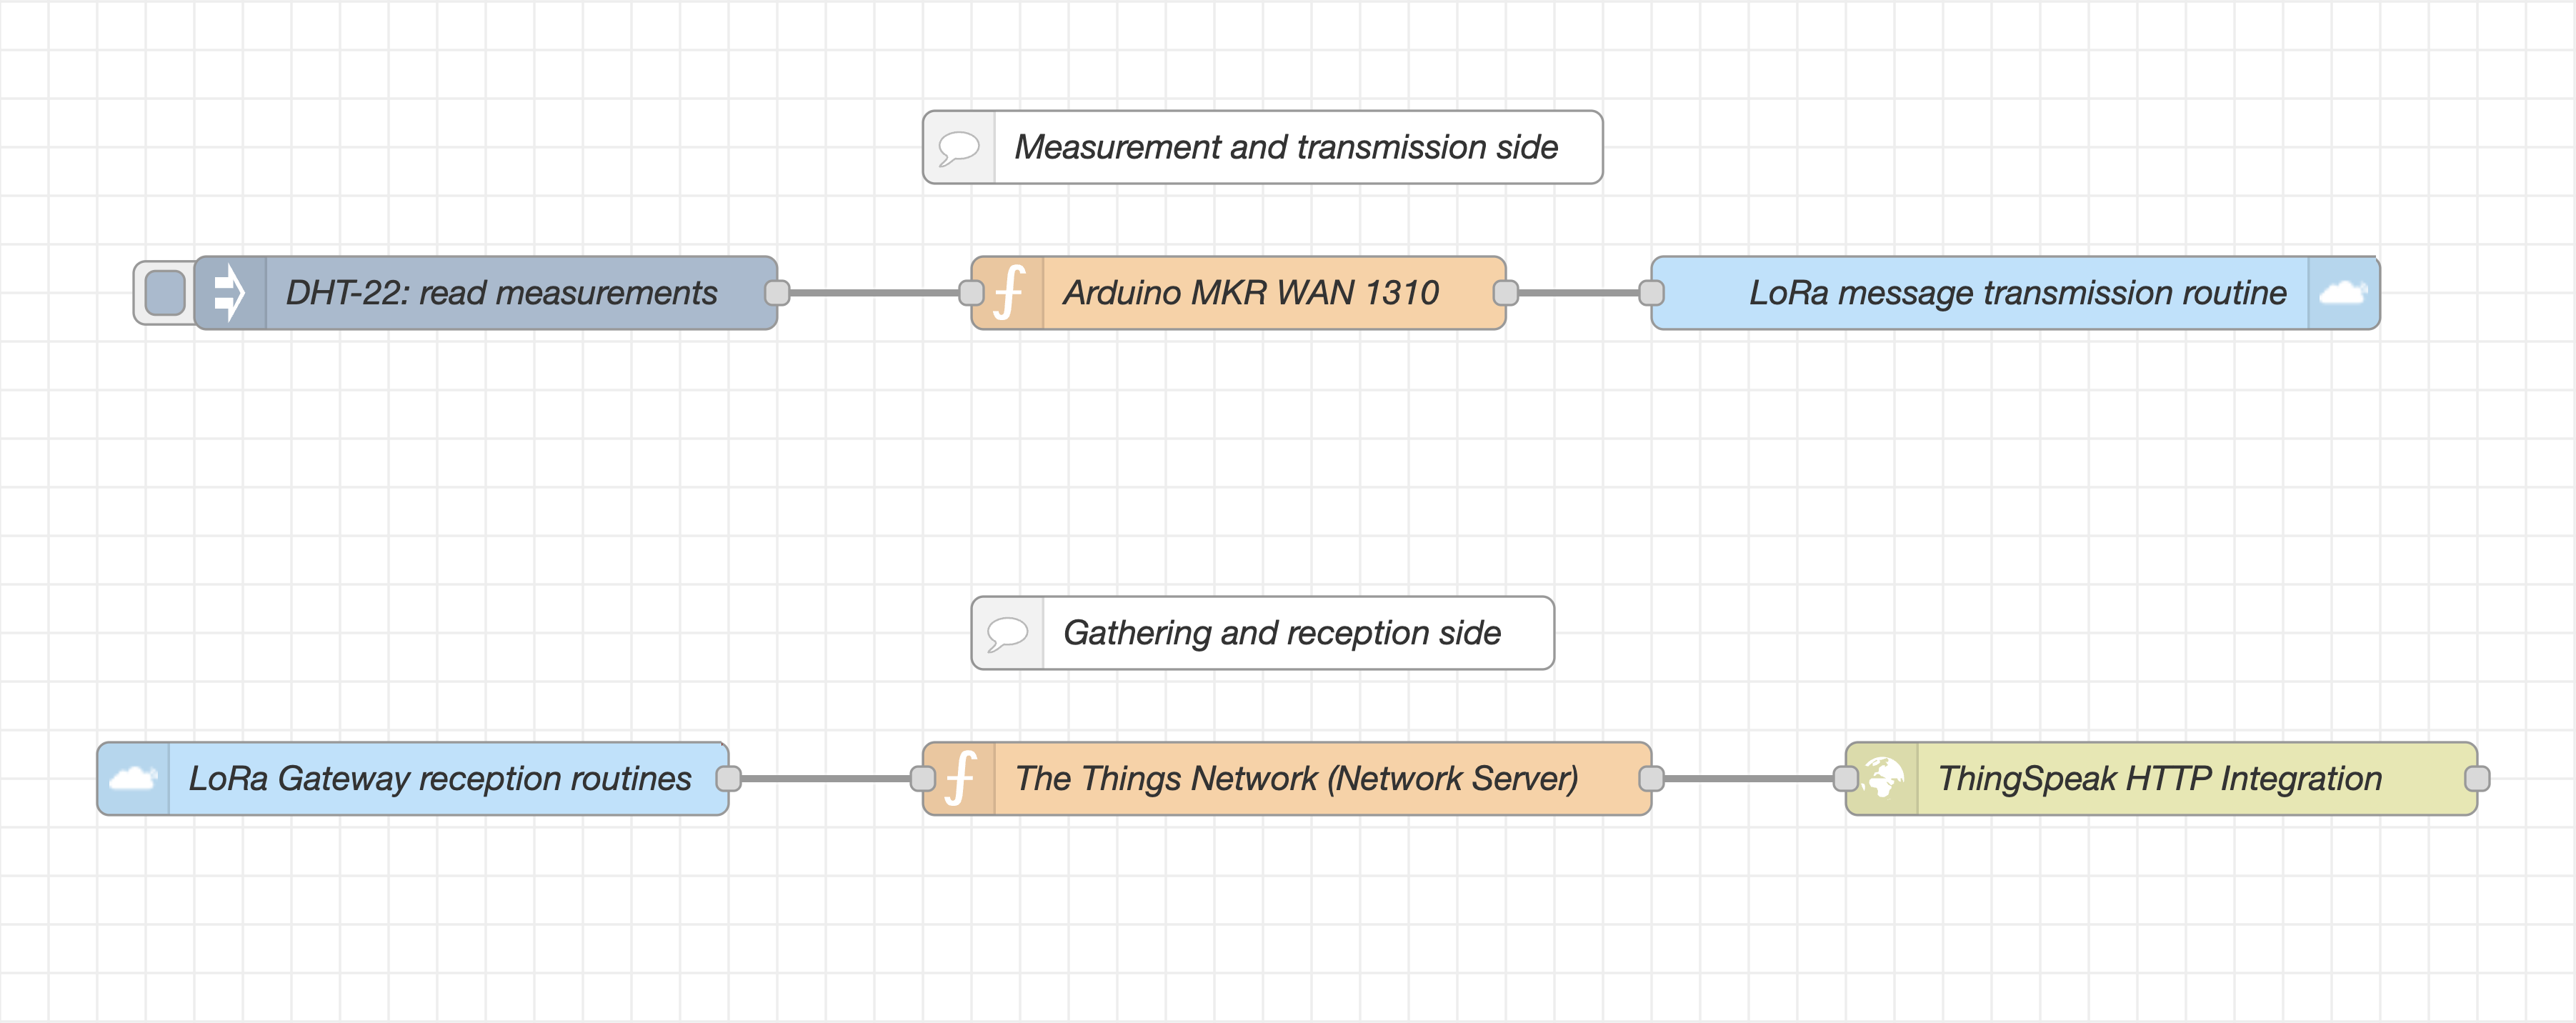
\includegraphics[width=18cm]{../res/node-red-eq2}


    \section{Question n. 3}\label{sec:question-n.-3}

    \subsection{Exercise text}\label{subsec:exercise-text3}

    Using the paper “Do LoRa Low-Power Wide-Area Networks Scale?” by M. Bor et al.
    and the LoRa simulator available at \href{https://www.lancaster.ac.uk/scc/sites/lora/lorasim.html}{LoRaSim}, your task is to reproduce Figure 5 and Figure 7 from the paper.

    \smallskip

    \begin{enumerate}
        \item Read the Paper: carefully study the relevant sections of the paper to understand the experimental setup, parameters, and key findings, especially those associated with Figures 5 and 7.
        \item Explore LoRaSim: familiarize yourself with how the LoRaSim simulator works.
        Understand its configuration options and how to run experiments that model LoRa network behavior.
        \item Reproduce the Figures
        \begin{enumerate}
            \item Use LoRaSim to replicate the simulations that produced Figure 5 and Figure 7.
            \item Ensure your simulation parameters (e.g., number of nodes, spreading factors, traffic load, transmission power, etc.) match those used in the original experiments as closely as possible.
            \item Present your results in the same format as the original figures for easy comparison.
        \end{enumerate}
    \end{enumerate}

    \subsection{Experiment sets}\label{subsec:experiment-sets}

    Let's start by first analyzing the paper: its aim is comparing some reasonably varied configurations of the LoRa operation modes, consisting of a mixture of Spreading Factors, Bandwidths, Coding Rates and Transmission Powers.

    \smallskip

    The outcomes of the chosen experiment sets line out the scaling characteristics of LoRa networks, investigating on capacity limits and developing models that describe the LoRa communication pattern and parametrize its behaviour.

    \smallskip

    To correlate the results to a real-world meaningful application and its scalability, a set of practical measurements has first been conducted on a real implementation, shaping a better understanding of the relationship among the varying parameters, shown in Figures 4, 5 and 7.

    \smallskip

    A \textsc{Configuration Set} is a set composed of Transmission Power, Carrier Frequency, Spreading Factor, Bandwidth, Carrier Rate, Transmission rate and Packet payload size.

    \smallskip

    For each cycle, we define the \textsc{Data Extraction Rate} (\textsc{DER}) parameter, which is related to the ratio of received messages to the total number of transmitted ones over a period of time, similarly to the concept of successful transmissions we introduced during laboratory lectures: being the \textsc{DER} intrinsically meaningful only from 0 to 1, the ideal \textsc{DER} value is the closest to 1 as possible.

    \smallskip

    \label{full-collision}
    Moreover, a \textsc{Full Collision Check} is performed, meaning that the full parametrical model of transmissions orthogonality is employed and checked for.

    \smallskip

    Finally, the chosen simulation duration is $\sim 58$ days.

    \medskip

    In the following, the set of conducted experiments is described.

    \begin{itemize}
        \item Figure 4: A simple setup consisting of $N$ nodes and one sink.

        A 20-byte packet is sent by each node every 16,7 minutes, to represent a realistic scenario.

        All nodes use the same configuration set, while three transmitter configurations are delineated:
        \begin{enumerate}
            \label{description-sn1}
            \item $SN_1$: The most robust LoRa transmitter settings, with the longest possible airtime (1712,13 ms).

            $SN_1$ has two definitions: one using Simple Channel Models and another one applying the LoRa-specific Channel Model.
            \item $SN_2$: The shortest possible airtime (7,07 ms).
            \item $SN_3$: The most common LoRaWAN deployment configuration setting.
        \end{enumerate}

        An exponential decrease of the \textsc{DER} is observed in most configurations with the growth of the number of nodes.

        The chosen split point is at $DER \geq 0,9$, to provide meaningful functionalities.

        In such a case, the default LoRaWAN configuration ($SN_3$) could host up to $N = 64$ nodes, while providing a communication range of $\sim 100\ meters$.

        A similar behaviour is observed for $SN_1$, while the extreme case ($SN_2$) provides small reliability and limits the transmission range to $\sim 37\ meters$.
        \item Figure 5: Dynamic communication parameter selection, $N$ nodes and one sink.

        Nodes are randomly placed but are guaranteed to reach the sink if the strongest configuration setting is used.

        Again, a 20-byte packet is sent by each node every 16,7 minutes, to represent a realistic scenario.
        \begin{enumerate}
            \item $SN_4$: Minimization of the airtime through Bandwidth, Spreading Factor and Carrier Rate configuration, but fixing the Transmit Power to $14\ dBm$.
            \item $SN_5$: Adds Transmit Power optimization on top of $SN_4$.
        \end{enumerate}
        Both $SN_4$ and $SN_5$, \hyperref[subsec:experimental-results]{as shown later}, provide a huge improvement to the default LoRaWAN deployment configuration ($SN_3$).

        In fact, up to $N = 1100$ can be supported, this time.

        However, these achievements turn out to be impractical, in a real-world scenario, as it relies on optimistic assumptions (no interference, little redundancy and no environment adaptation).
        \item Figure 7: Multiple nodes and sinks.

        Again, a 20-byte packet is sent by each node every 16,7 minutes, to represent a realistic scenario.

        The chosen experiment set, this time, consists of only $SN_1$, \hyperref[description-sn1]{the same one described earlier}.

        As multiple sinks are now present, a new placement strategy has to be applied.

        The chosen one relies on some simple geometrical considerations that are aimed at equally spacing a multiple number of sinks and, compatibly, the multiple nodes.

        Results, \hyperref[subsec:experimental-results]{also replicated later}, show that the increase in the number of sinks relates to a corresponding increase in the \textsc{DER}.

        Somewhat counter-intuitively, in fact, the increase in the number of sinks does not have a visible impact on reliability (saturation) of the nodes.
    \end{itemize}

    \subsection{LoRaSim: the LoRa implementation simulator}\label{subsec:lorasim:-the-lora-implementation-simulator}

    As a compound to the provided paper, an automated tool has been developed to run a similar set of experiments, aimed at determining the final DER, given a varying number of nodes (and sinks) and tuning some configuration settings according to the experimental runs.

    \smallskip

    It consists of a group of \textsc{Python 2} scripts: the interesting ones, for our experimental runs, are \texttt{loraDir.py} and \texttt{loraDirMulBS.py}, that respectively cover the single and multi-sink cases.

    \smallskip

    The simulator accepts the following parameters:

    \begin{itemize}
        \item Nodes: number $N$ of nodes to include.
        \item AvgSend: inverse of the transmission rate: average sending interval, in milliseconds.
        \item SimTime: simulation duration.
        \item BaseStations: number $M$ of sinks to include.
        \item Collision: enables the \textsc{Full Collision Check}, as \hyperref[full-collision]{mentioned earlier}.
        \item Experiment: an integer index identifying the characteristics of each experimental run.

        The matching between experimental runs and the \hyperref[subsec:experiment-sets]{experiment sets} delineated by the paper dissertation is also sketched.
        \begin{enumerate}
            \setcounter{enumi}{-1}
            \item Use the settings with the slowest datarate (Spreading Factor = SF12, Bandwidth = 125 kHz, Coding Rate = 4/8), similarly to $SN_1$.
            \item Similar to experiment 0, but uses a random choice of three transmit frequencies.
            This experimental run does not match a complete experiment set.
            \item Use the settings with the fastest data rate (Spreading Factor = SF6, Bandwidth = 500 kHz, Coding Rate = 4/5), similarly to $SN_2$.
            \item Optimize the setting per node based on the distance to the gateway, similarly to $SN_4$.
            \item Use the settings as defined in LoRaWAN (Spreading Factor = SF12, Bandwidth = 125 kHz, Coding Rate = 4/5), similarly to $SN_3$.
            \item Similar to experiment 3, but also optimizes the transmission power, similarly to $SN_5$.
        \end{enumerate}
    \end{itemize}

    \subsubsection{The updated version}

    Following the paper's release, a couple of bugs have been made clear by the scientific community, resulting in an update to the \textsc{LoRaSim} simulator.

    \smallskip

    These updates were, in particular, aimed at correcting the use of logarithms in the path-loss model and revisiting the presumably too optimistic approach taken by the simulator in overestimating the network's throughput.

    \smallskip

    The paper's authors released an updated version of both \href{https://www.research.lancs.ac.uk/portal/en/publications/do-lora-lowpower-widearea-networks-scale(83d93e9d-8d77-4927-8f9c-cdca397fe355).html}{the paper} and \href{https://www.lancaster.ac.uk/scc/sites/lora/lorasim-20170710.tgz}{the simulator}.

    \smallskip

    However, since both versions can be interpreted as a solid result and being the outcomes unchanged, they are both taken into consideration when replicating them.

    \medskip

    Note that, of course, the updated reference is the most accurate, with respect to the real-world implementation.

    \medskip

    The old version is replicated starting from the updated one, as shown in the following.

    \begin{minted}{bash}
# Update LoRaSim with its modified old version (see notes)
sudo apt-get install -y sed

cp lorasim/loraDir.py lorasim/loraDir-old.py
cp lorasim/loraDirMulBS.py lorasim/loraDirMulBS-old.py

# Remove lines 116 and 117 (corresponding to the collisions sub-estimation)
sed -i '116,+1d;' lorasim/loraDir-old.py

# Replace natural logarithms with base-10 logarithm
sed -i 's/math.log10/math.log/g' lorasim/loraDir-old.py

# Remove lines 107 and 108 (corresponding to the collisions sub-estimation)
sed -i '107,+1d;' lorasim/loraDirMulBS-old.py

# Replace natural logarithms with base-10 logarithm
sed -i 's/math.log10/math.log/g' lorasim/loraDirMulBS-old.py
    \end{minted}

    \newpage

    \subsection{Experimental results}\label{subsec:experimental-results}

    In the following, a comparison between the plot results of Figure 5 and 7 is provided for both the old and updated versions.

    \begin{figure}[H]
        \centering
        \subfloat[\centering \textsc{Python} simulation]{{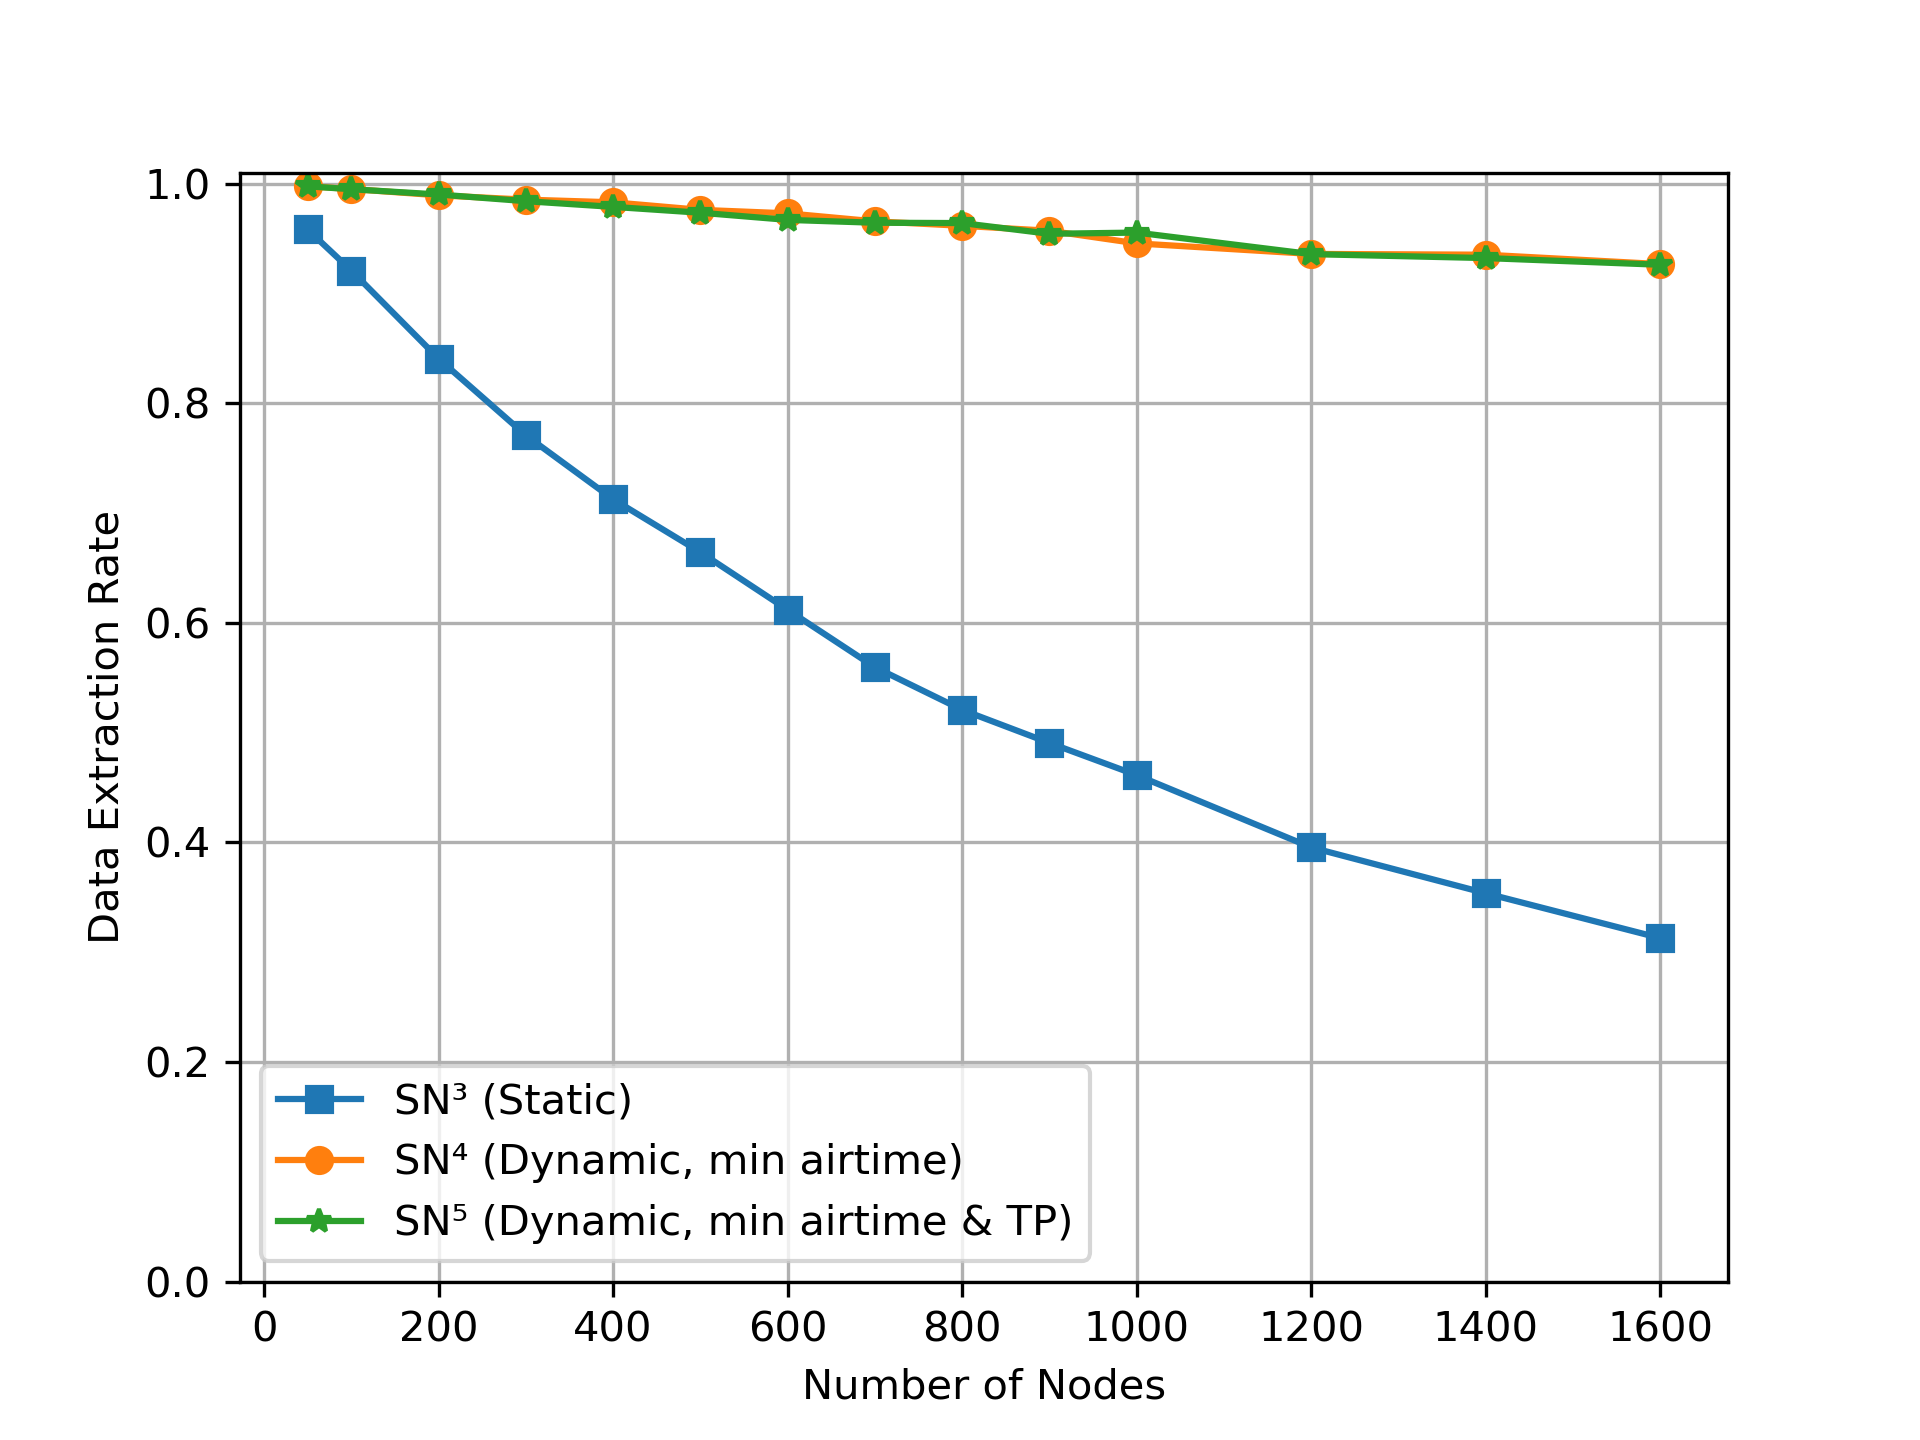
\includegraphics[width=8.3cm]{../res/python-f5-old} }}
        \qquad
        \subfloat[\centering Paper]{{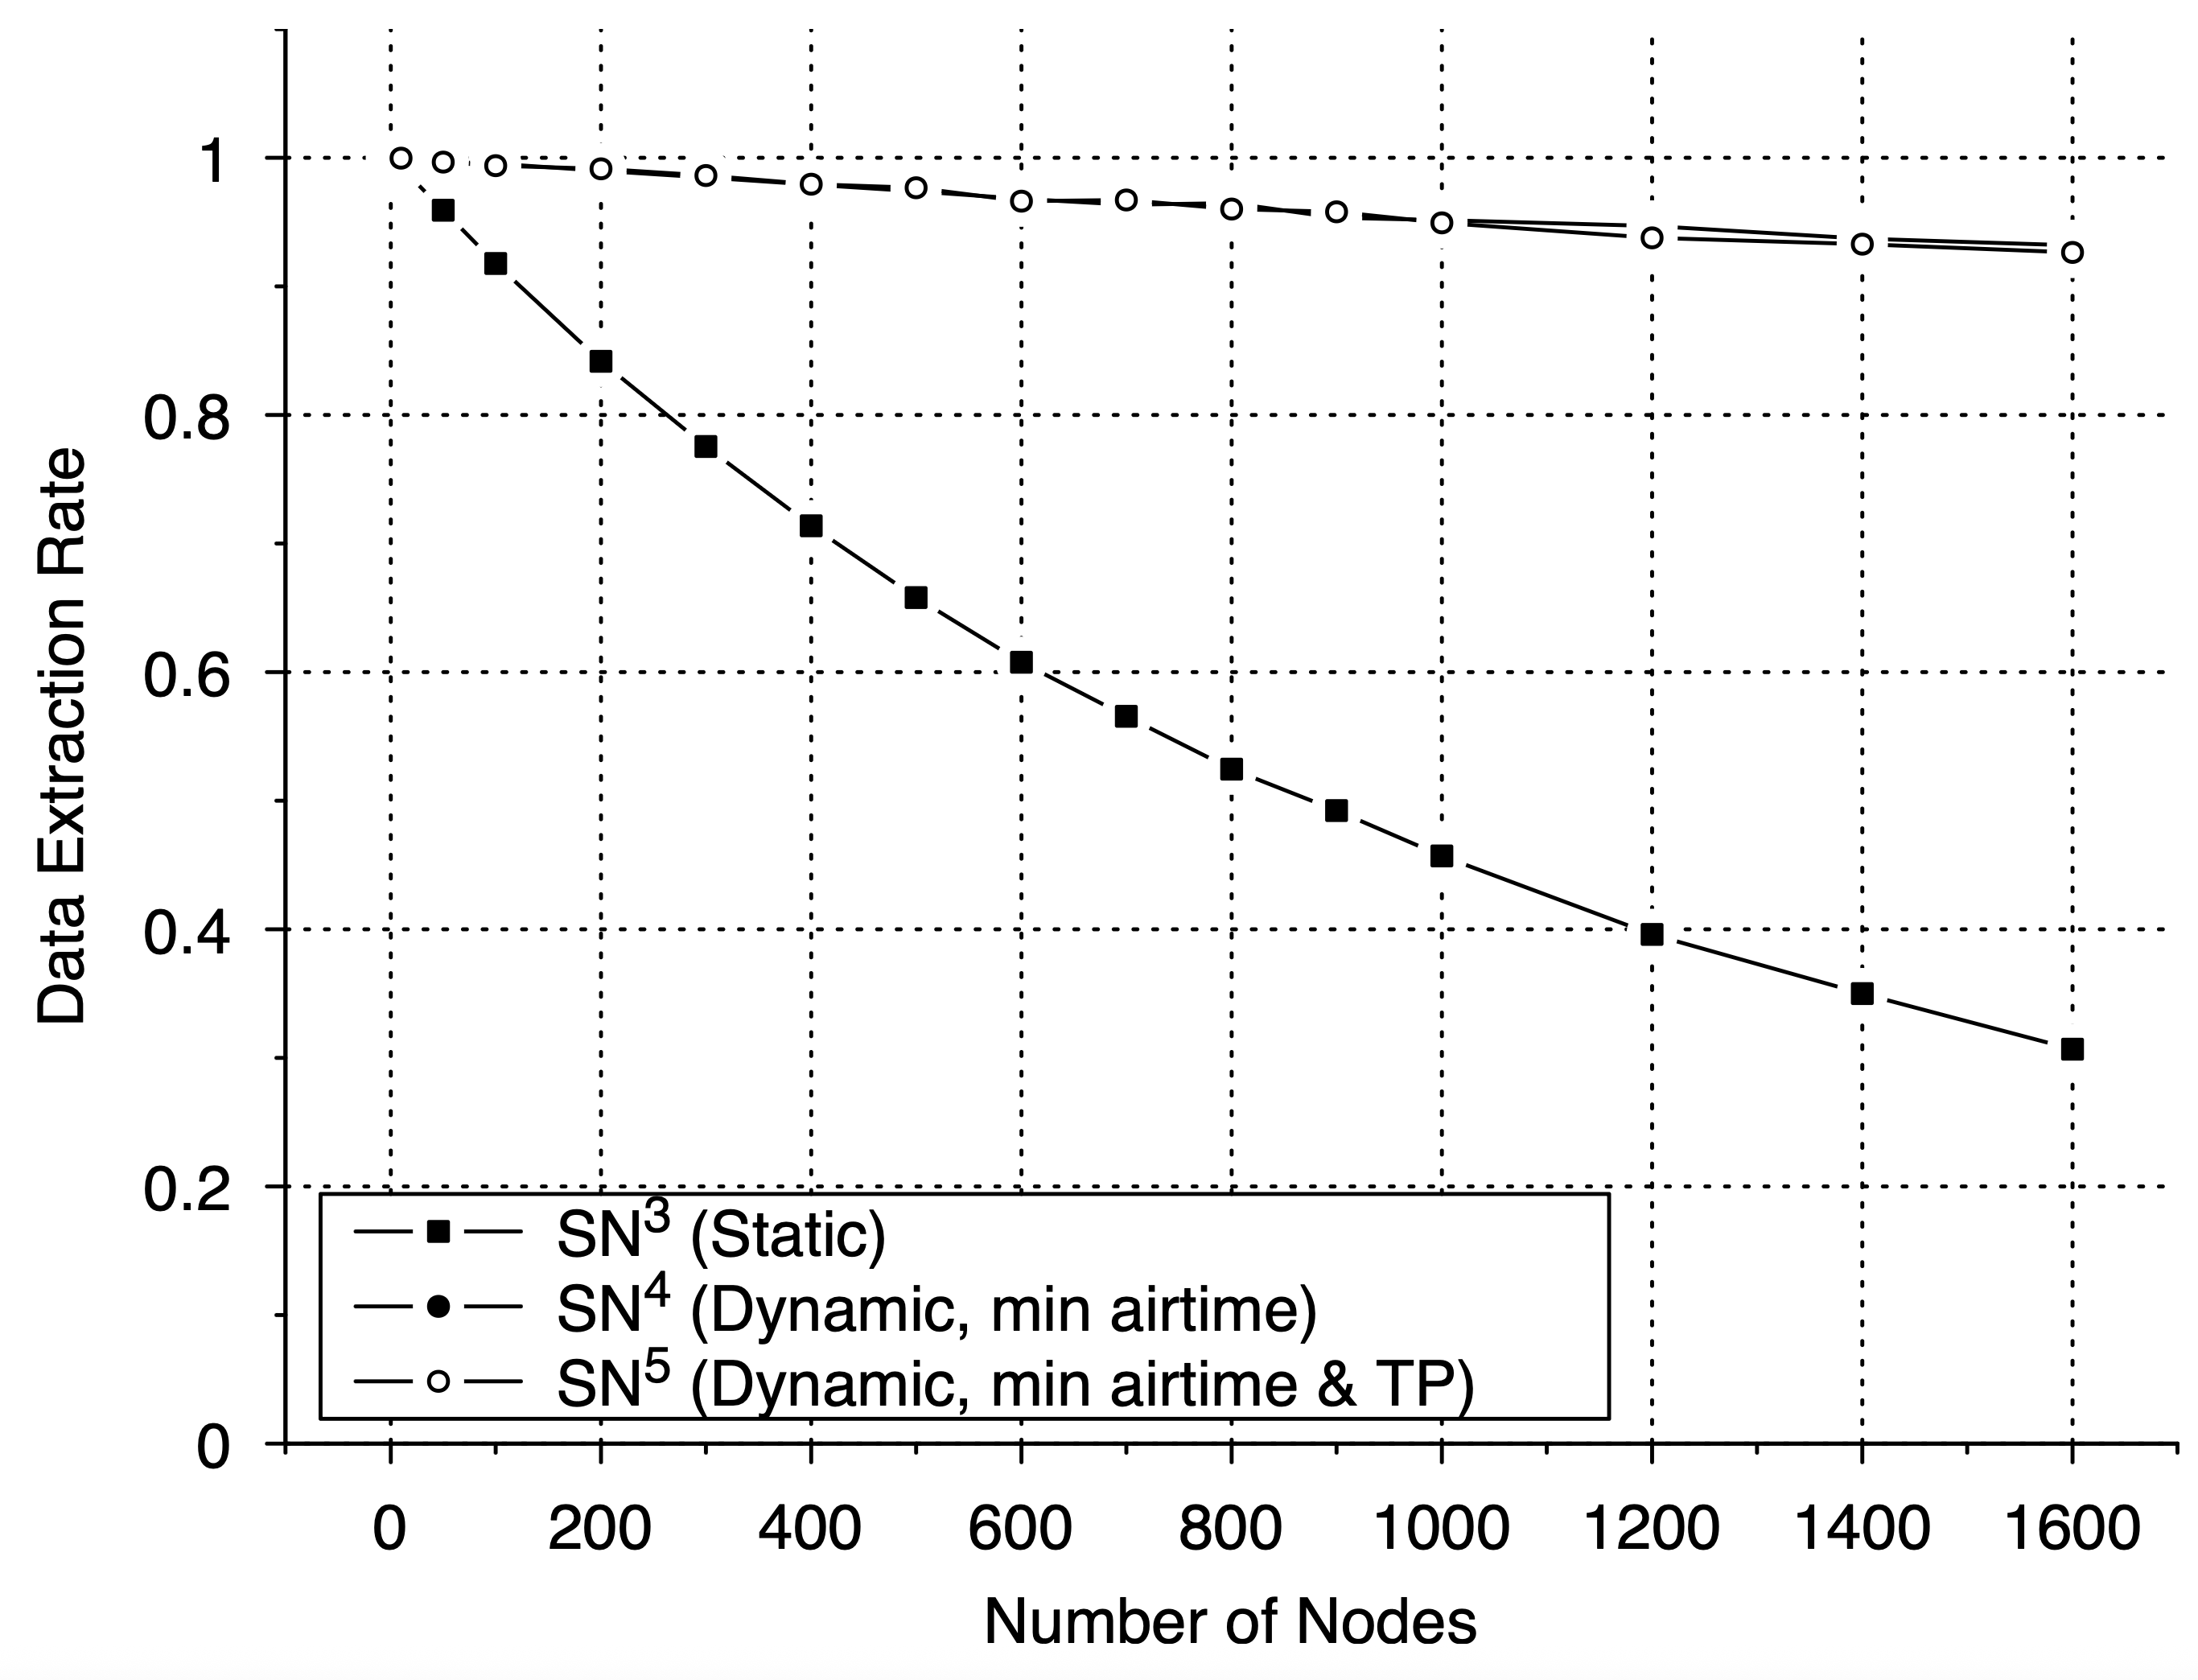
\includegraphics[width=8cm]{../res/paper-f5-old} }}
        \caption{Comparison: Figure 5, old version of the simulator}
        \label{fig:comparison-f5-old}
    \end{figure}

    Both $SN_4$ and $SN_5$ provide a huge improvement to the default LoRaWAN deployment configuration.

    \smallskip

    In fact, up to $N = 1100$ can be accomodated, according to the requirement imposing $DER \geq 0,9$.

    \smallskip

    However, these achievements turn out to be impractical, in a real-world scenario, as it relies on optimistic assumptions (no interference, little redundancy and no environment adaptation).

    \begin{figure}[H]
        \centering
        \subfloat[\centering \textsc{Python} simulation]{{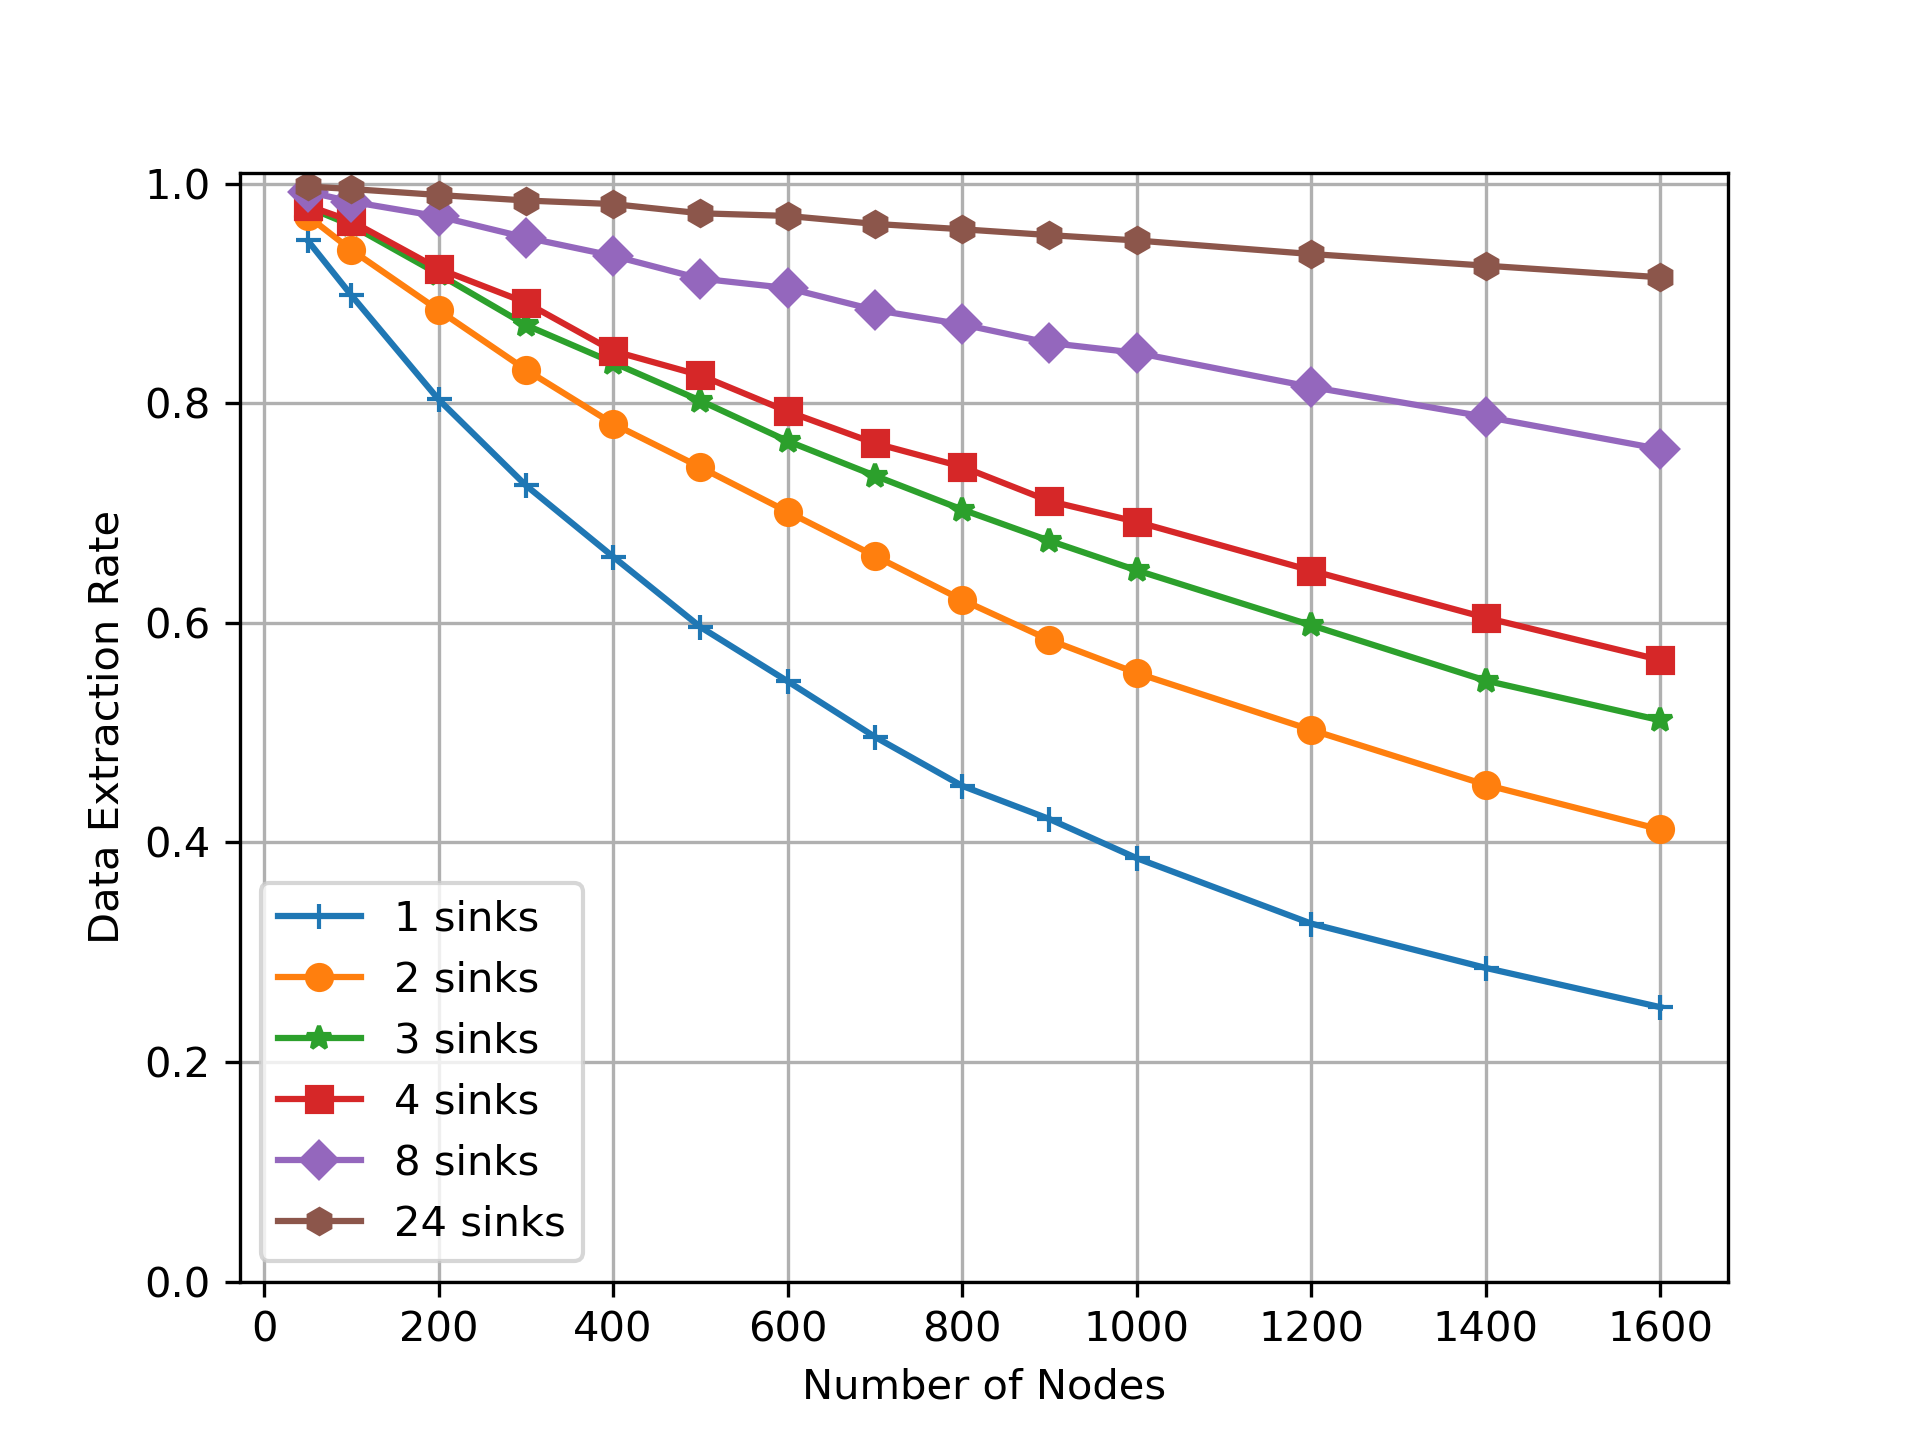
\includegraphics[width=8.3cm]{../res/python-f7-old} }}
        \qquad
        \subfloat[\centering Paper]{{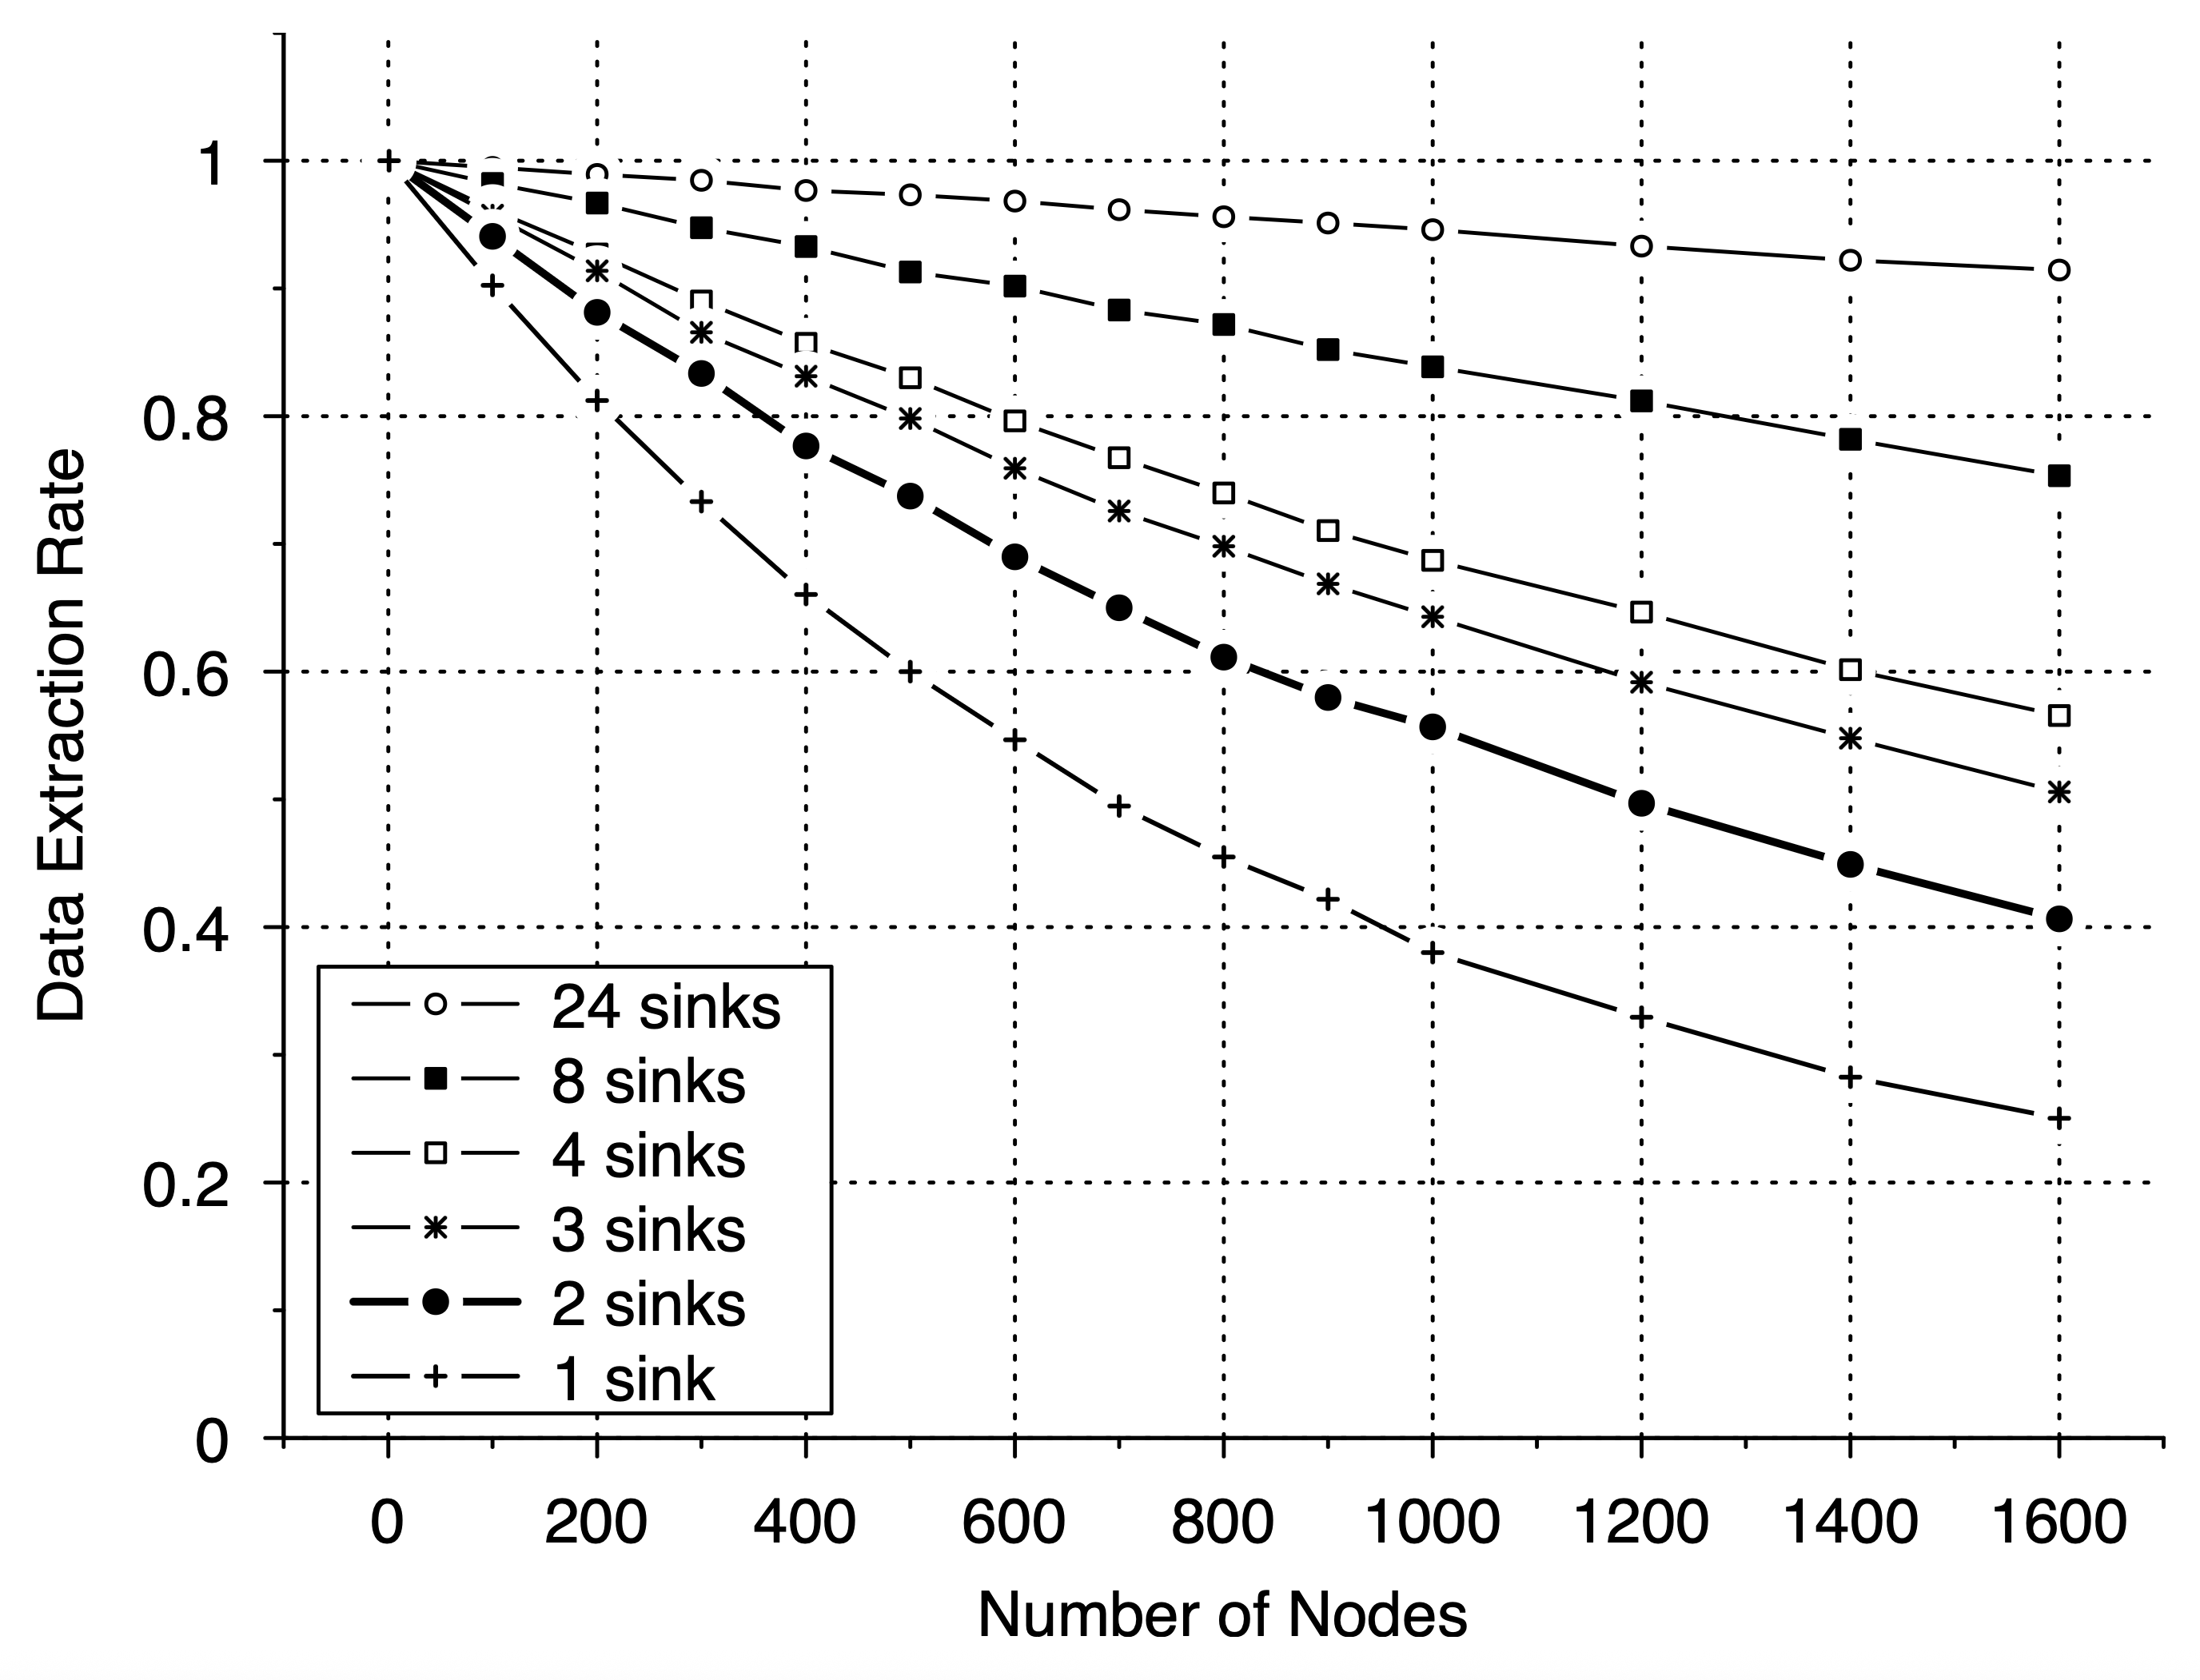
\includegraphics[width=8cm]{../res/paper-f7-old} }}
        \caption{Comparison: Figure 7, old version of the simulator}
        \label{fig:comparison-f7-old}
    \end{figure}

    Results show that the increase in the number of sinks relates to a corresponding increase in the \textsc{DER}.

    \smallskip

    Somewhat counter-intuitively, in fact, the increase in the number of sinks does not have a visible impact on reliability (saturation) of the nodes.

    \smallskip

    The same also applies to the results produced by the updated version of the simulator.

    \begin{figure}[H]
        \centering
        \subfloat[\centering \textsc{Python} simulation]{{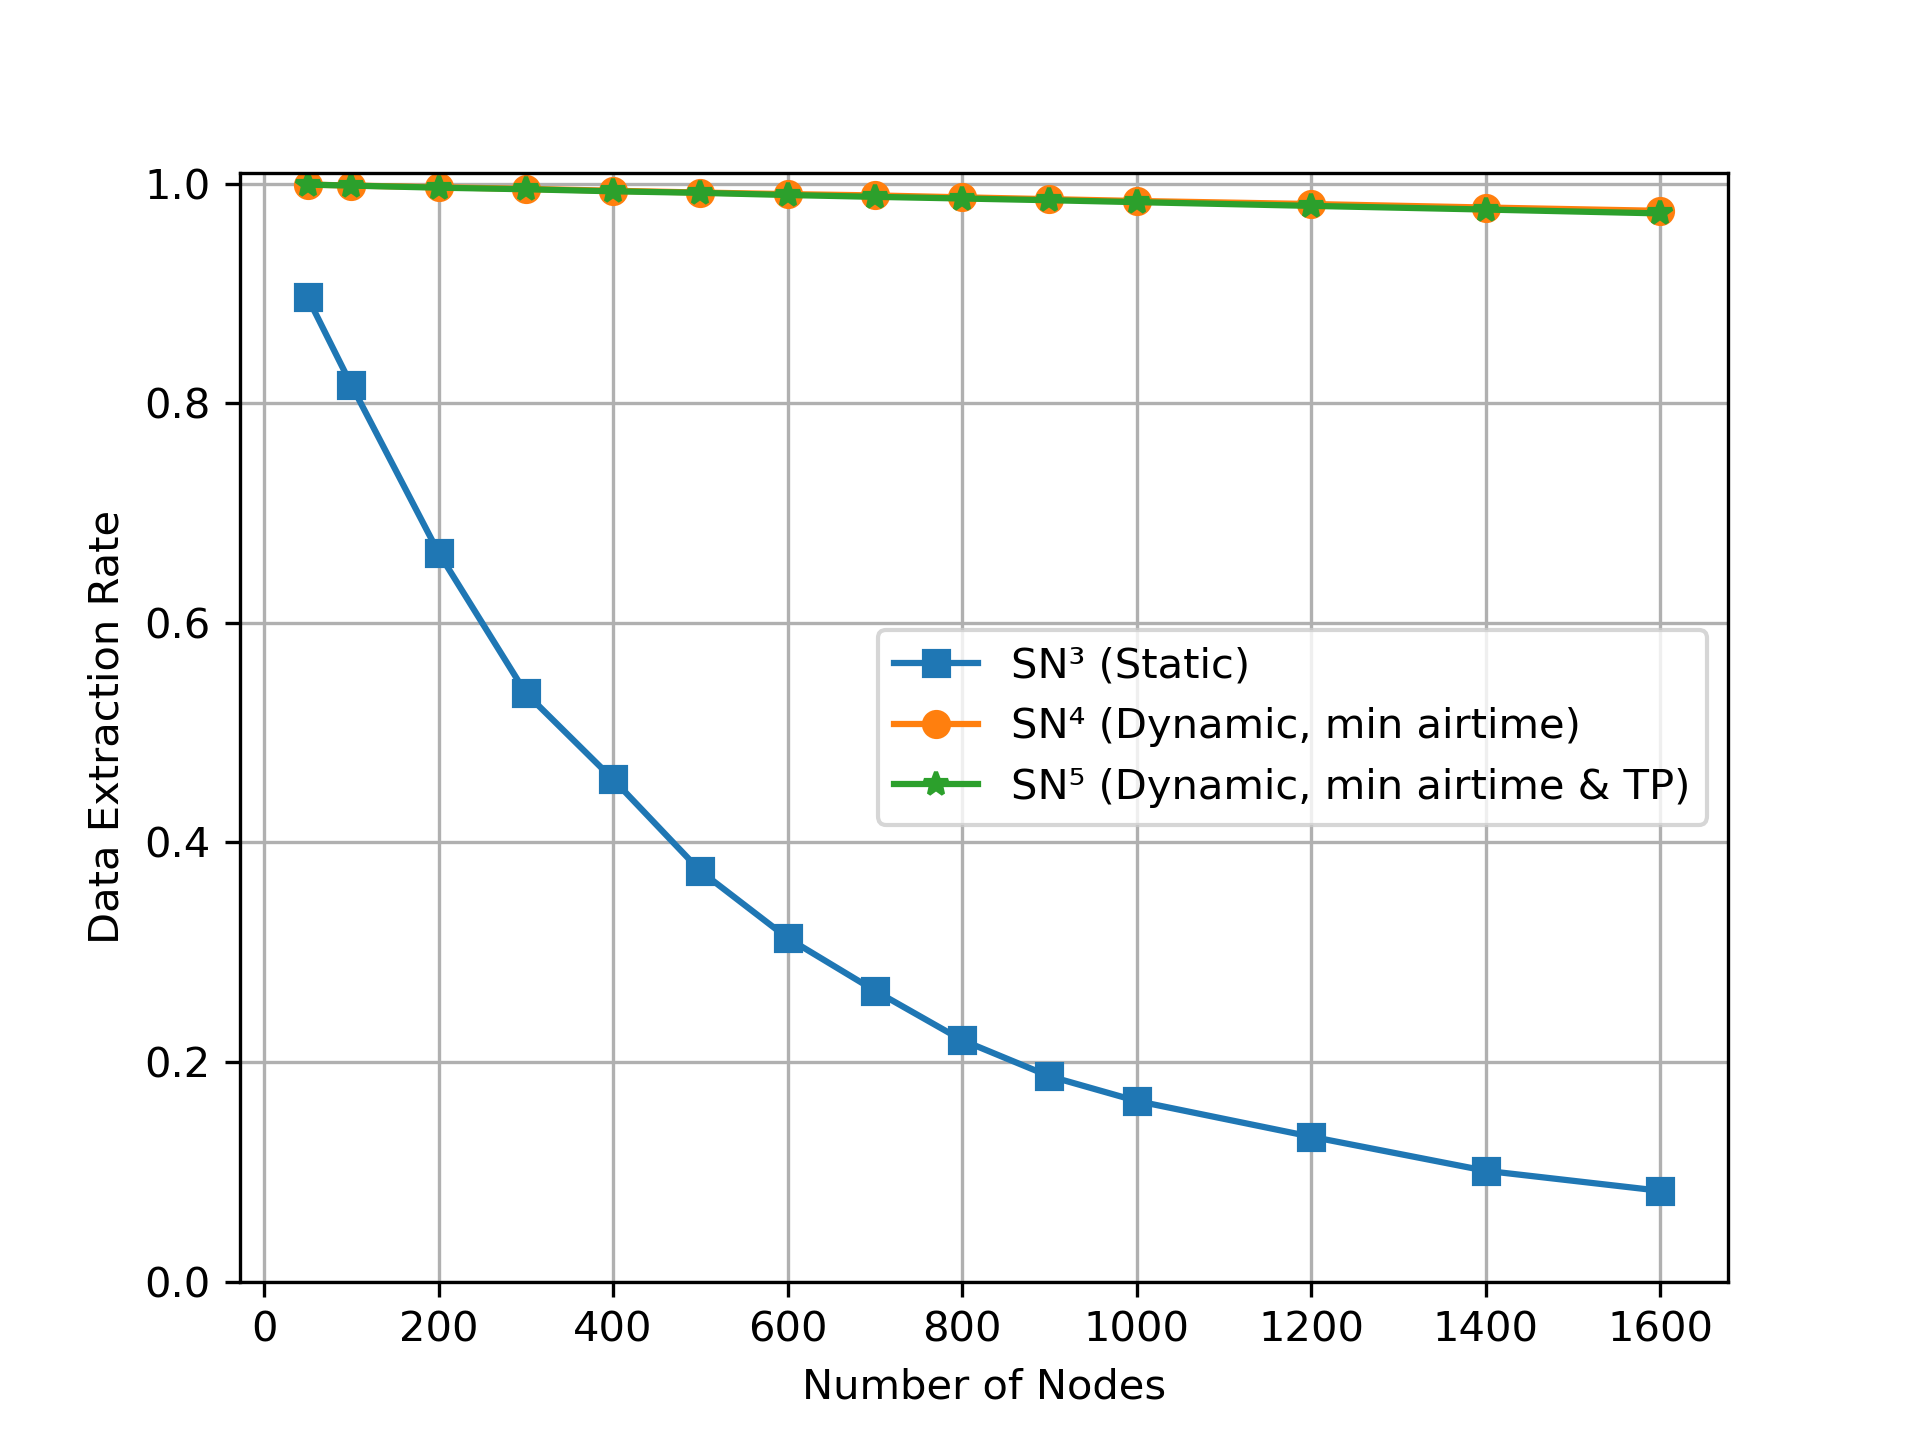
\includegraphics[width=8.3cm]{../res/python-f5-updated} }}
        \qquad
        \subfloat[\centering Paper]{{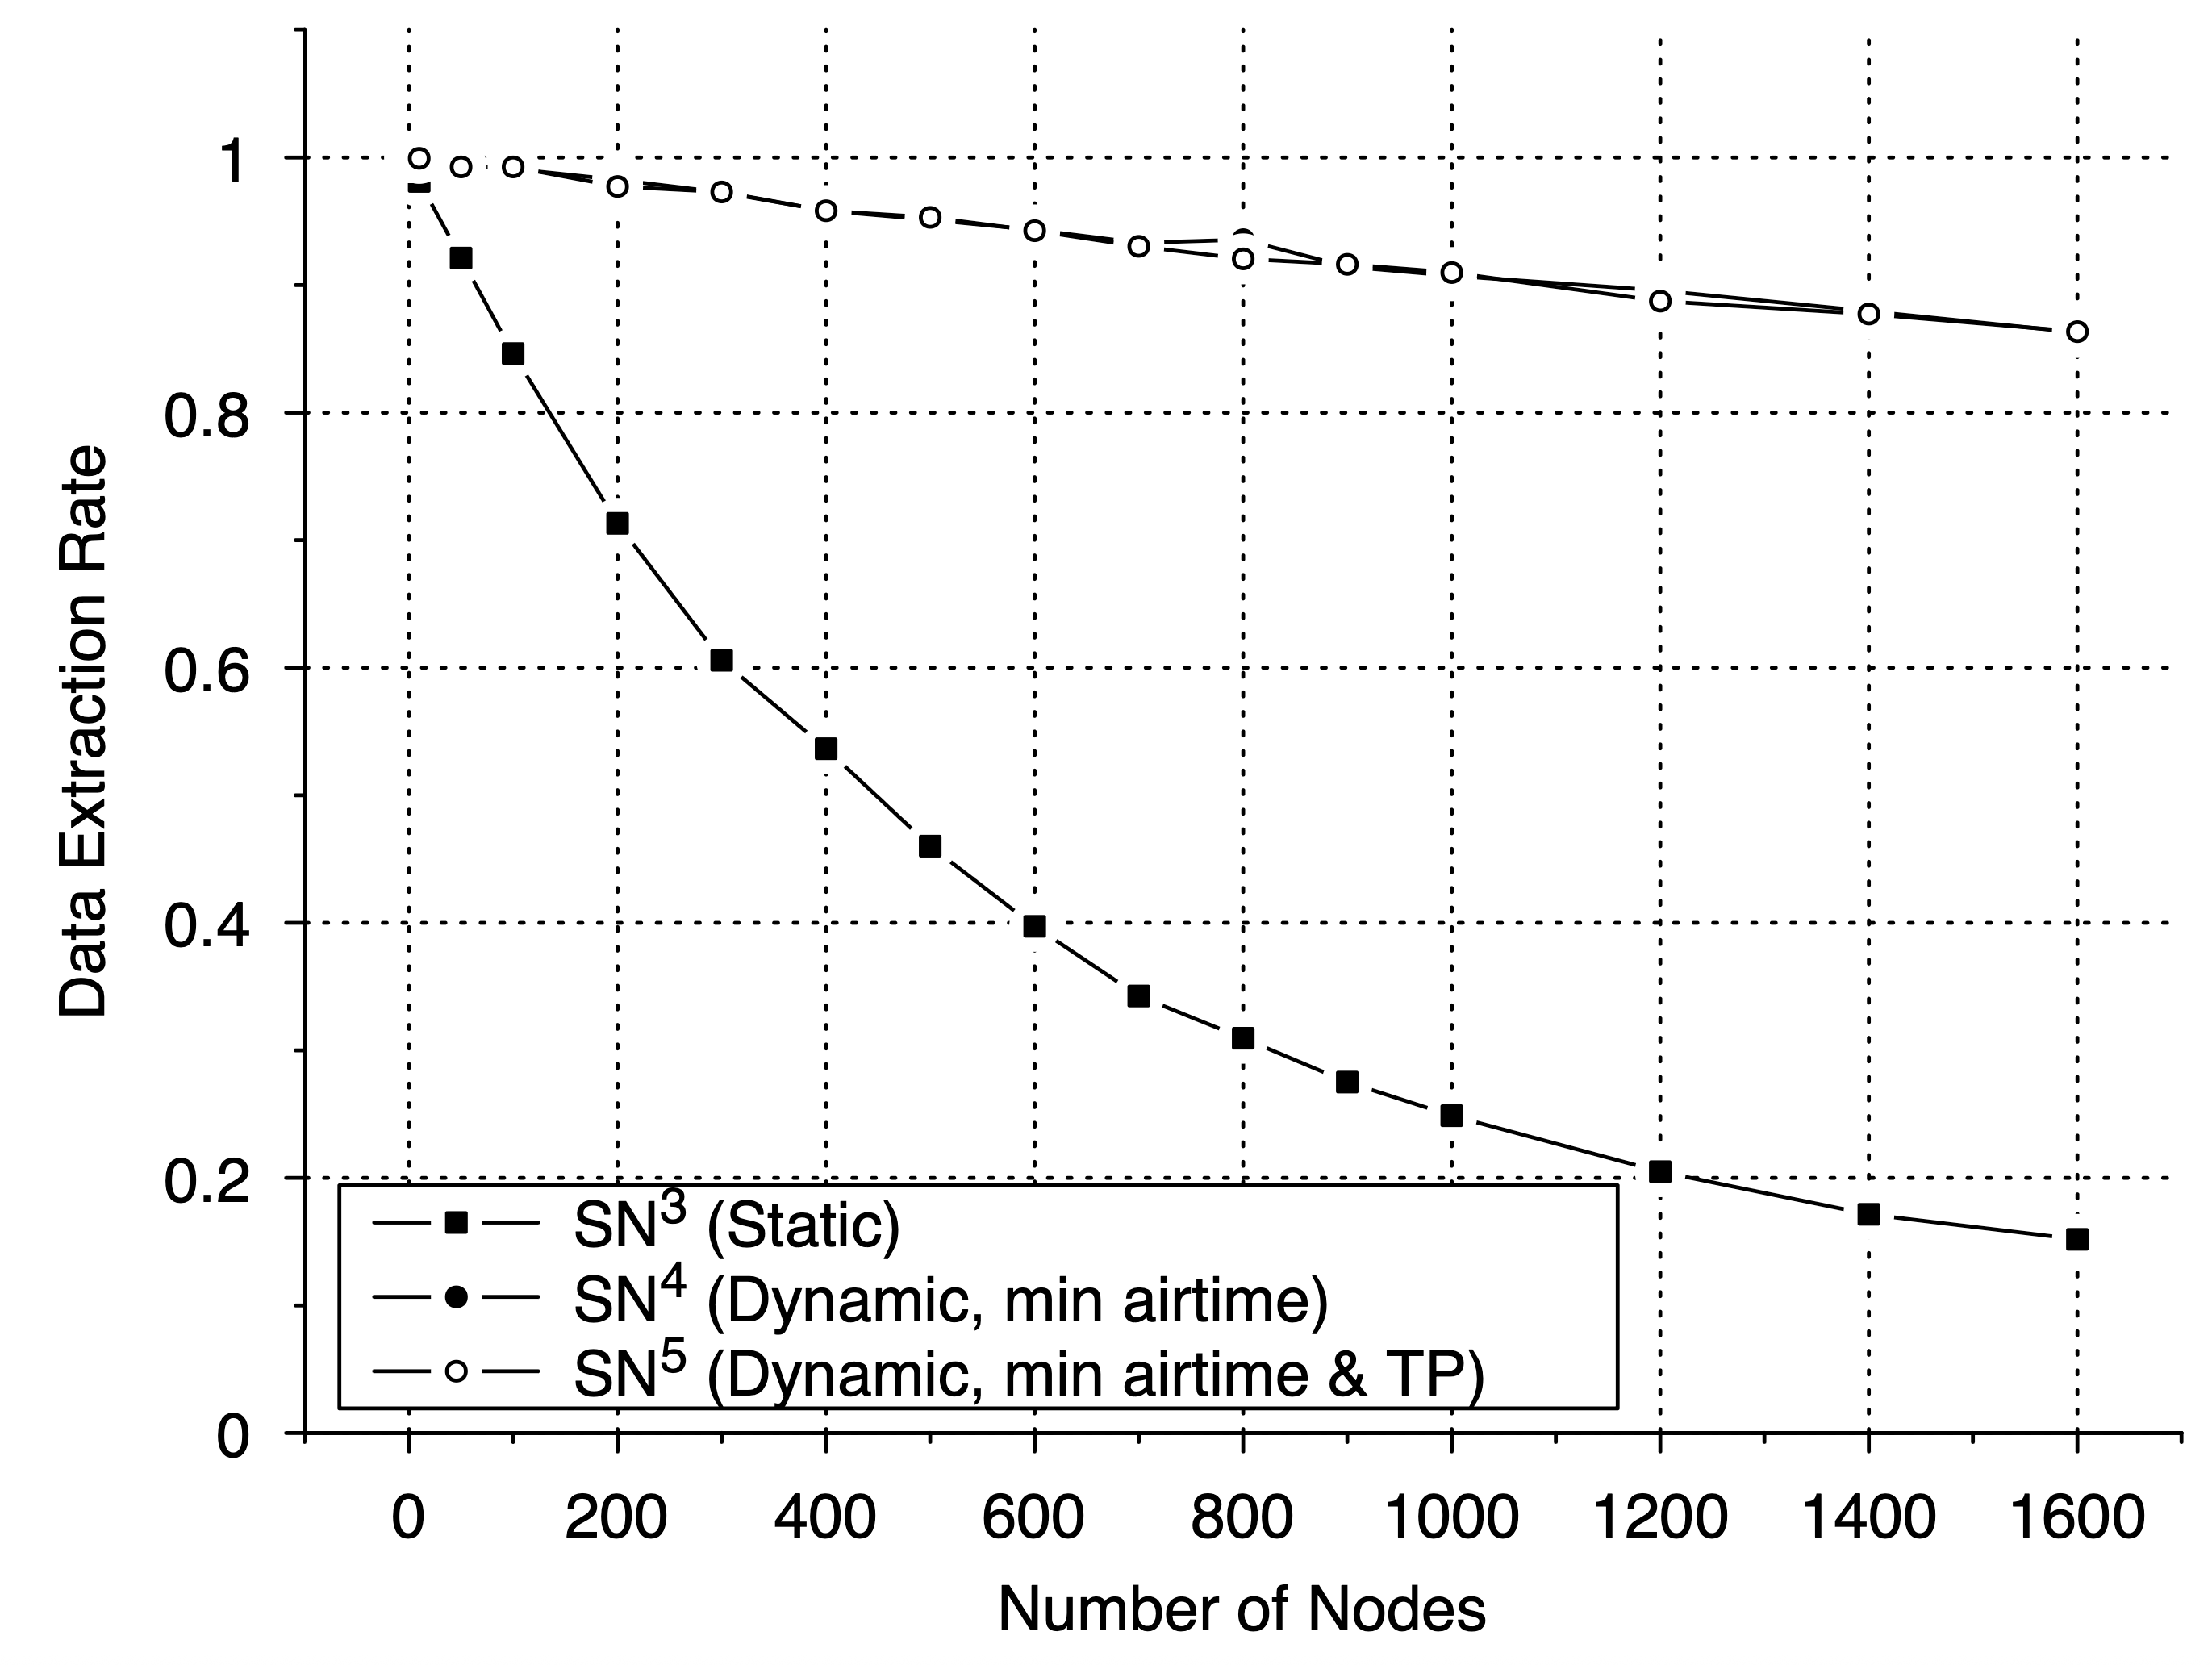
\includegraphics[width=8cm]{../res/paper-f5-updated} }}
        \caption{Comparison: Figure 5, updated version of the simulator}
        \label{fig:comparison-f5-updated}
    \end{figure}

    \begin{figure}[H]
        \centering
        \subfloat[\centering \textsc{Python} simulation]{{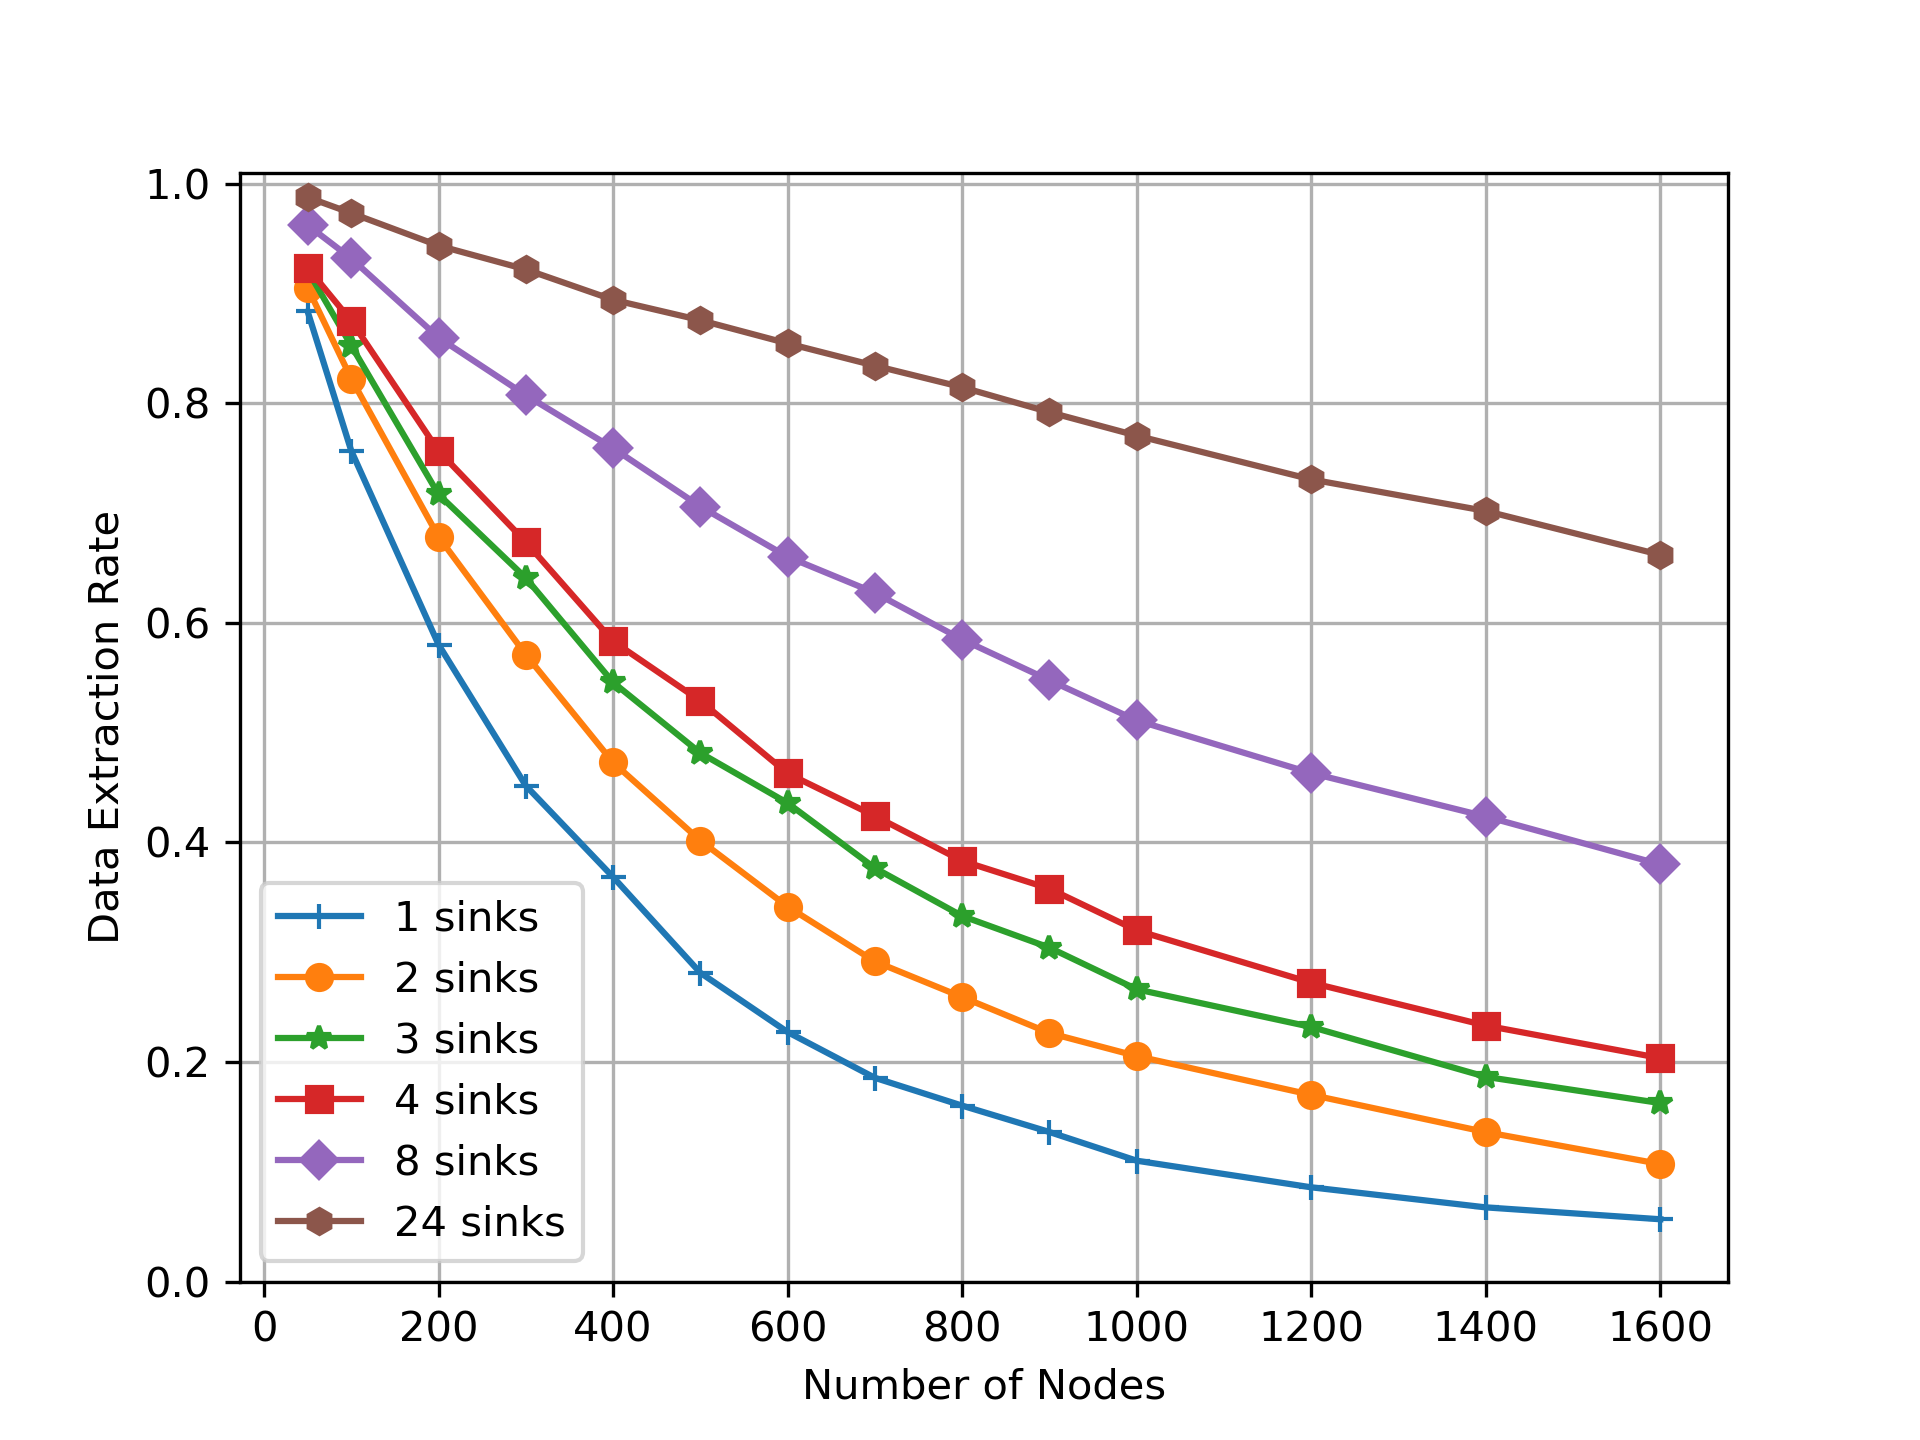
\includegraphics[width=8.3cm]{../res/python-f7-updated} }}
        \qquad
        \subfloat[\centering Paper]{{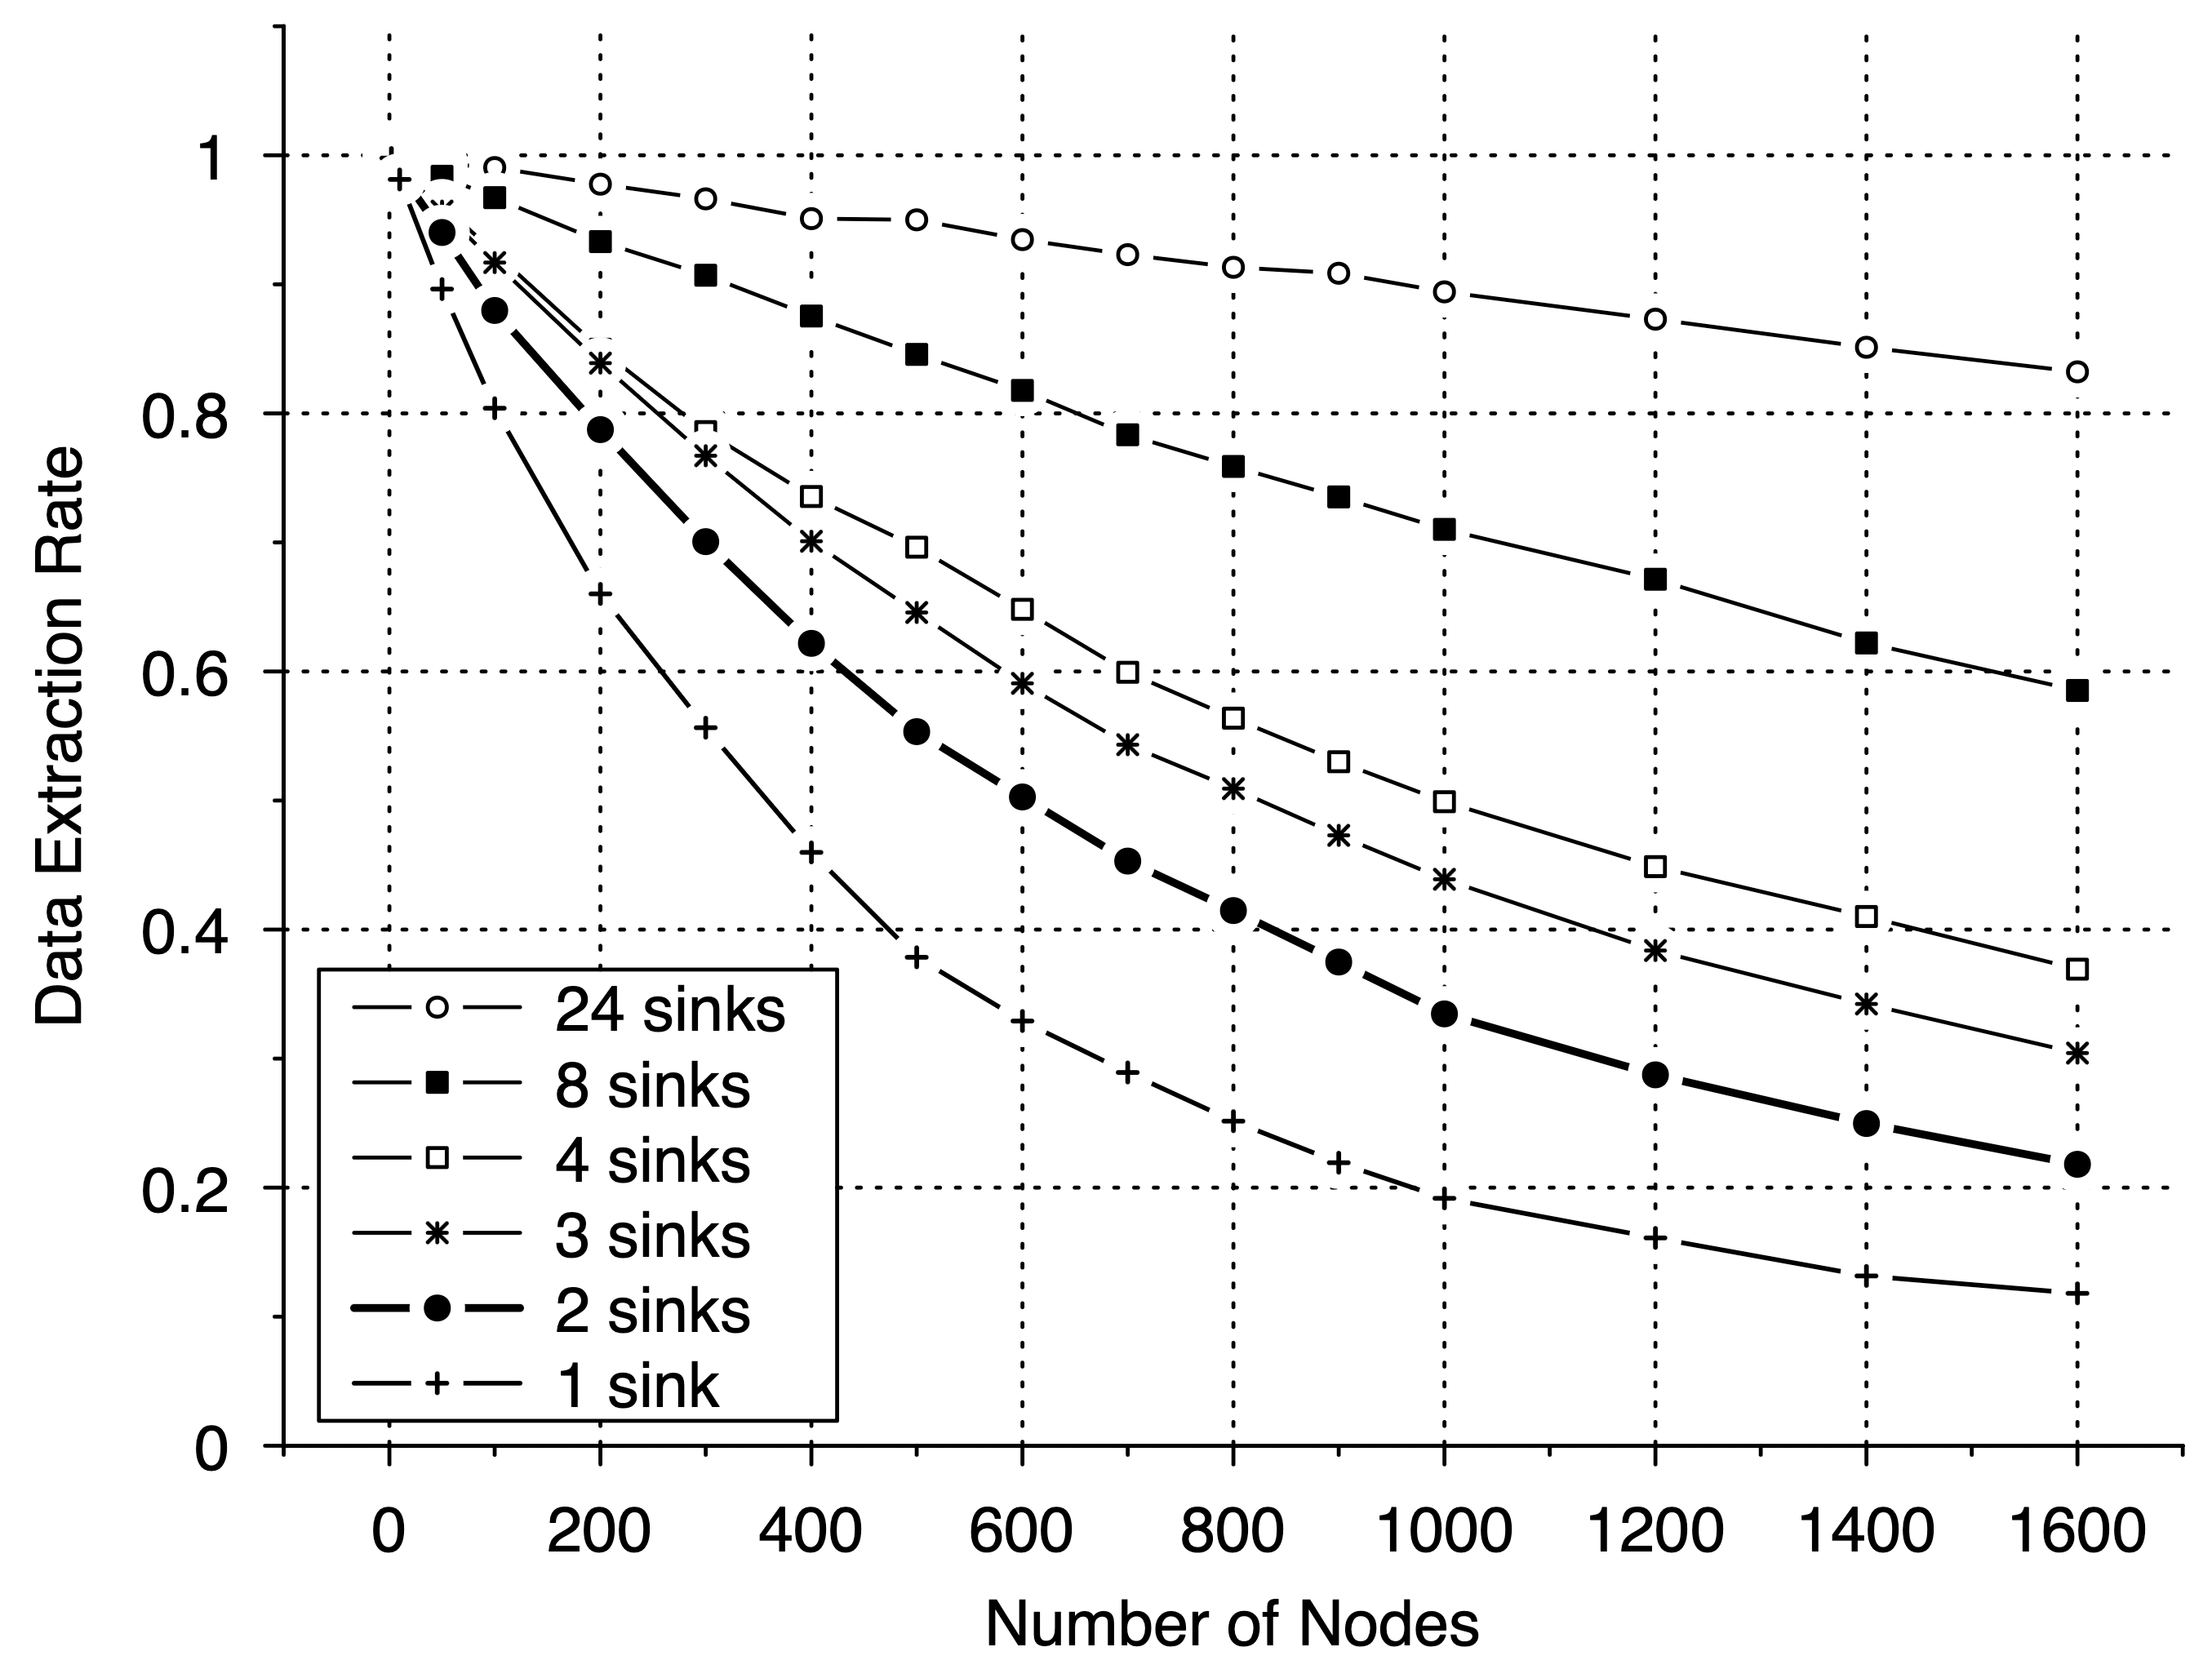
\includegraphics[width=8cm]{../res/paper-f7-updated} }}
        \caption{Comparison: Figure 7, updated version of the simulator}
        \label{fig:comparison-f7-updated}
    \end{figure}

    \subsection{Implementation details (in Python)}\label{subsec:implementation-details-(in-python)}

    \subsubsection*{Common libraries import}

    \begin{minted}{Python}
import pandas as pd
import math
import matplotlib.pyplot as plt
import subprocess
import os
import re
import glob
import shutil
    \end{minted}

    \subsubsection*{Simulation primitives}

    Note that the simulator's output is heavily verbose: it must be discarded.

    \smallskip

    Otherwise, for higher configurations, it will fill out the machine's memory and crash.

    \begin{minted}{Python}
# Simulation output directories (see notes)
UPDATED_VARIANT_DIR = "updated"
OLD_VARIANT_DIR = "old"


def simulate(n_nodes, tx_rate, exp, duration, collisions=True, old=False):
    env = os.environ.copy()
    env["MPLBACKEND"] = "Agg"

    # Old version discriminant (see notes)
    if old:
        old = "-old"
    else:
        old = ""

    # Final output directory (for simulation outputs)
    output_directory = OLD_VARIANT_DIR if old else UPDATED_VARIANT_DIR

    # Use subprocess.run to execute the command and capture output
    result = subprocess.run(
        [
            "python2",
            (
                f"/lorasim/loraDir{old}.py"
                if not COLAB
                else f"{os.getcwd()}/lorasim/loraDir{old}.py"
            ),
            str(int(n_nodes)),
            str(int(tx_rate)),
            str(int(exp)),
            str(int(duration)),
            str(int(collisions)),
        ],
        cwd=f"{os.getcwd()}/{output_directory}",
        env=env,
        # The simulator produces a heavily verbose output: it must be discarded.
        # Otherwise, for higher configurations, it will fill out the machine's memory!
        # The standard simulator's output is discarded, while the errors stream is kept.
        stdout=subprocess.DEVNULL,
        stderr=subprocess.STDOUT,
        # capture_output=True,
        # text=True,  # Capture output as text
    )

    # Print the output
    # print(result.stdout)
    # print(result.stderr)


def simulate_multisink(
    n_nodes, tx_rate, exp, duration, base_stations, collisions=True, old=False
):
    env = os.environ.copy()
    env["MPLBACKEND"] = "Agg"

    # Old version discriminant (see notes)
    if old:
        old = "-old"
    else:
        old = ""

    # Final output directory (for simulation outputs)
    output_directory = OLD_VARIANT_DIR if old else UPDATED_VARIANT_DIR

    # Use subprocess.run to execute the command and capture output
    result = subprocess.run(
        [
            "python2",
            (
                f"/lorasim/loraDirMulBS{old}.py"
                if not COLAB
                else f"{os.getcwd()}/lorasim/loraDirMulBS{old}.py"
            ),
            str(int(n_nodes)),
            str(int(tx_rate)),
            str(int(exp)),
            str(int(duration)),
            str(int(base_stations)),
            str(int(collisions)),
        ],
        cwd=f"{os.getcwd()}/{output_directory}",
        env=env,
        # The simulator produces a heavily verbose output: it must be discarded.
        # Otherwise, for higher configurations, it will fill out the machine's memory!
        # The standard simulator's output is discarded, while the errors stream is kept.
        stdout=subprocess.DEVNULL,
        stderr=subprocess.STDOUT,
        # capture_output=True,
        # text=True,  # Capture output as text
    )

    # Print the output
    # print(result.stdout)
    # print(result.stderr)


# Der in aloha defined as S/G = e^(-2G)
def aloha_der(n_nodes, t):
    rate = 1e-6
    return math.exp(-2 * n_nodes * rate * t)
    \end{minted}

    \subsubsection*{Environment cleanup and management primitives}

    \begin{minted}{Python}
def reformat_multisink(directory="."):
    # Regular expression that matches files ending in BS{number}.dat
    pattern_file = re.compile(r".*BS\d+\.dat$")

    # Get all .dat files
    dat_files = glob.glob(os.path.join(directory, "*.dat"))

    # Filter for the matching ones
    files = [f for f in dat_files if pattern_file.match(f)]

    for path in files:
        # Read contents and locally store them
        with open(path, "r") as file:
            lines = file.readlines()

        # Update status flag
        status = False

        for i, line in enumerate(lines):
            if line.startswith("# "):
                # Remove the # extra space (for the format alignment)
                lines[i] = "#" + line[2:]
                status = True

        # Update file contents with the reformatted one
        if status:
            with open(path, "w") as file:
                file.writelines(lines)


def simulation_outputs(directory="."):
    # Get all .dat files
    dat_files = glob.glob(os.path.join(directory, "*.dat"))
    # And also computation outputs from the multi-basestation case
    bs_file = glob.glob(os.path.join(directory, "basestation.txt"))
    nodes_file = glob.glob(os.path.join(directory, "nodes.txt"))
    # And finally output figures
    output_figures = glob.glob(os.path.join(directory, "figure*.png"))
    return dat_files + bs_file + nodes_file + output_figures


def cleanup_environment(directory="."):
    for f in simulation_outputs(directory):
        os.remove(f)


# Automatically invoke cleanup of the environment
cleanup_environment(f"./{UPDATED_VARIANT_DIR}")
cleanup_environment(f"./{OLD_VARIANT_DIR}")

try:
    os.mkdir(f"./{UPDATED_VARIANT_DIR}")
    os.mkdir(f"./{OLD_VARIANT_DIR}")
except:
    pass
    \end{minted}

    \subsubsection*{Simulation — Figure 5}

    \begin{minted}{Python}
# Problem data
# one packet of length L every 16,7 min = 16.7 * 60 * 1000 ms
transmission_rate = 16.7 * 60 * 1000
# 58 days simulation (see notes)
duration = 58 * 24 * 60 * 60 * 1000
# Enable the full collisions tracing model (see notes)
full_collision_model = True

n_nodes = [50, 100, 200, 300, 400, 500, 600, 700, 800, 900, 1000, 1200, 1400, 1600]

# Experiments set
experiments = [4, 3, 5]

# Iterate on all the interesting node configurations
for nodes in n_nodes:
    print(
        f"Simulating experiments n. {experiments[0]}, {experiments[1]} and {experiments[2]} on {nodes} nodes"
    )
    for exp in experiments:
        # Updated variant
        simulate(nodes, transmission_rate, exp, duration, full_collision_model, False)
        # Old variant
        simulate(nodes, transmission_rate, exp, duration, full_collision_model, True)
    \end{minted}

    \label{output-fig5}
    \begin{tcolorbox}
        Simulating experiments n. 4, 3 and 5 on 50 nodes

        Simulating experiments n. 4, 3 and 5 on 100 nodes

        Simulating experiments n. 4, 3 and 5 on 200 nodes

        Simulating experiments n. 4, 3 and 5 on 300 nodes

        Simulating experiments n. 4, 3 and 5 on 400 nodes

        Simulating experiments n. 4, 3 and 5 on 500 nodes

        Simulating experiments n. 4, 3 and 5 on 600 nodes

        Simulating experiments n. 4, 3 and 5 on 700 nodes

        Simulating experiments n. 4, 3 and 5 on 800 nodes

        Simulating experiments n. 4, 3 and 5 on 900 nodes

        Simulating experiments n. 4, 3 and 5 on 1000 nodes

        Simulating experiments n. 4, 3 and 5 on 1200 nodes

        Simulating experiments n. 4, 3 and 5 on 1400 nodes

        Simulating experiments n. 4, 3 and 5 on 1600 nodes
    \end{tcolorbox}

    \subsubsection*{Extract simulation results files}

    \begin{minted}{Python}
data = []
data_old = []
for exp in experiments:
    data.append(pd.read_csv(f"{UPDATED_VARIANT_DIR}/exp{exp}.dat", sep=" "))
    data_old.append(pd.read_csv(f"{OLD_VARIANT_DIR}/exp{exp}.dat", sep=" "))
    \end{minted}

    \subsubsection*{Data preparation}

    \begin{minted}{Python}
for d in data:
    d["der"] = (d["nrTransmissions"] - d["nrCollisions"]) / d["nrTransmissions"]

for d in data_old:
    d["der"] = (d["nrTransmissions"] - d["nrCollisions"]) / d["nrTransmissions"]

labels = [
    "SN3 (Static)",
    "SN4 (Dynamic, min airtime)",
    "SN5 (Dynamic, min airtime & TP)",
]

markers = ["s", "o", "*"]

# Explicit assertion: datasets and their labels are coherent in size
assert len(data) == len(data_old)
assert len(data) == len(labels)

# Example of the resulting data
data[0].head()
data_old[0].head()
    \end{minted}

    \subsubsection*{Data plot, updated variant}

    \begin{minted}{Python}
plt.figure(dpi=300)  # higher resolution plot
for i in range(0, len(data)):
    # Plot labelled data sets: Number of nodes on the X axis and Data Extraction Rate on the Y axis
    plt.plot(data[i]["#nrNodes"], data[i]["der"], marker=markers[i], label=labels[i])
plt.xlabel("Number of Nodes")
plt.ylabel("Data Extraction Rate")
# Valid Y range is from 0 to 1 (an extra is included for representation spacing)
plt.ylim(0, 1 + 0.01)
plt.legend()
plt.grid()
plt.savefig(f"{UPDATED_VARIANT_DIR}/figure5.png")
plt.show()
    \end{minted}

    \subsubsection*{Data plot, old variant}

    \begin{minted}{Python}
plt.figure(dpi=300)  # higher resolution plot
for i in range(0, len(data_old)):
    # Plot labelled data sets: Number of nodes on the X axis and Data Extraction Rate on the Y axis
    plt.plot(
        data_old[i]["#nrNodes"], data_old[i]["der"], marker=markers[i], label=labels[i]
    )
plt.xlabel("Number of Nodes")
plt.ylabel("Data Extraction Rate")
# Valid Y range is from 0 to 1 (an extra is included for representation spacing)
plt.ylim(0, 1 + 0.01)
plt.legend()
plt.grid()
plt.savefig(f"{OLD_VARIANT_DIR}/figure5.png")
plt.show()
    \end{minted}

    \subsubsection*{Simulation — Figure 7}

    \begin{minted}{Python}
# Problem data
# one packet of length L every 16,7 min = 16.7 * 60 * 1000 ms
transmission_rate = 16.7 * 60 * 1000
n_sinks = [1, 2, 3, 4, 8, 24]  # base stations (sinks)
# 58 days simulation (see notes)
duration = 58 * 24 * 60 * 60 * 1000
# Enable the full collisions tracing model (see notes)
full_collision_model = True

n_nodes = [50, 100, 200, 300, 400, 500, 600, 700, 800, 900, 1000, 1200, 1400, 1600]

# Experiments set consists only of a common setting (see notes)
experiment = 0

# Iterate on all the interesting node (and sink) configurations
for sink in n_sinks:
    for nodes in n_nodes:
        print(
            f"Simulating experiment n. {experiment} on {nodes} nodes and {sink} sinks"
        )
        # Updated variant
        simulate_multisink(
            nodes,
            transmission_rate,
            experiment,
            duration,
            sink,
            full_collision_model,
            False,
        )
        # Old variant
        simulate_multisink(
            nodes,
            transmission_rate,
            experiment,
            duration,
            sink,
            full_collision_model,
            True,
        )

# Reformat results for the plot sub-computations, for both the updated and old cases
reformat_multisink(f"./{UPDATED_VARIANT_DIR}")
reformat_multisink(f"./{OLD_VARIANT_DIR}")
    \end{minted}

    The output is suppressed, being heavily verbose and very similar to \hyperref[output-fig5]{the one of Figure 5}.

    \subsubsection*{Extract simulation results files}

    \begin{minted}{Python}
data = []
data_old = []
for sink in n_sinks:
    data.append(
        pd.read_csv(f"{UPDATED_VARIANT_DIR}/exp{experiment}BS{sink}.dat", sep=" ")
    )
    data_old.append(
        pd.read_csv(f"{OLD_VARIANT_DIR}/exp{experiment}BS{sink}.dat", sep=" ")
    )
    \end{minted}

    \subsubsection*{Data preparation}

    \begin{minted}{Python}
# Each sink configuration has its own dataset
labels = [f"{s} sinks" for s in n_sinks]

markers = ["+", "o", "*", "s", "D", "h"]

# Explicit assertion: datasets and their labels are coherent in size
assert len(data) == len(data_old)
assert len(data) == len(labels)

# Example of the resulting data
data[0].head()
data_old[0].head()
    \end{minted}

    \subsubsection*{Data plot, updated variant}

    \begin{minted}{Python}
plt.figure(dpi=300)  # higher resolution plot
for i in range(0, len(data)):
    # Plot labelled data sets: Number of nodes on the X axis and Data Extraction Rate on the Y axis
    plt.plot(data[i]["#nrNodes"], data[i]["DER"], marker=markers[i], label=labels[i])
plt.xlabel("Number of Nodes")
plt.ylabel("Data Extraction Rate")
# Valid Y range is from 0 to 1 (an extra is included for representation spacing)
plt.ylim(0, 1 + 0.01)
plt.legend()
plt.grid()
plt.savefig(f"{UPDATED_VARIANT_DIR}/figure7.png")
plt.show()
    \end{minted}

    \subsubsection*{Data plot, old variant}

    \begin{minted}{Python}
plt.figure(dpi=300)  # higher resolution plot
for i in range(0, len(data_old)):
    # Plot labelled data sets: Number of nodes on the X axis and Data Extraction Rate on the Y axis
    plt.plot(data_old[i]["#nrNodes"], data_old[i]["DER"], marker=markers[i], label=labels[i])
plt.xlabel("Number of Nodes")
plt.ylabel("Data Extraction Rate")
# Valid Y range is from 0 to 1 (an extra is included for representation spacing)
plt.ylim(0, 1 + 0.01)
plt.legend()
plt.grid()
plt.savefig(f"{OLD_VARIANT_DIR}/figure7.png")
plt.show()
    \end{minted}

    \subsection{Optionally: a Docker container}\label{subsec:optionally:-a-docker-container}

    The \textsc{LoRaSim} simulator and its revised variant need installation, on the local system, of both \textsc{Python 2}, for the simulator and \textsc{Python 3} for the notebook's execution.

    \smallskip

    Therefore, to provide a common abstraction layer, a specifically crafted \textsc{Dockerfile} is included in the repository, alongside a full \textsc{Development Container} environment, providing all the most common \textsc{Jupyter notebooks} requirements and \textsc{LoRaSim}.

    \smallskip

    When built, it can be used to serve as an interpreter for the project, integrating it with the embedded \textsc{Python Conda} environment.

    \begin{minted}{text}
FROM --platform=linux/amd64 quay.io/jupyter/base-notebook

#### INSTALL DEPENDENCIES ####
RUN conda update --all --yes \
    && conda install --yes notebook nest-asyncio pandas numpy scapy matplotlib scikit-learn

#### INSTALL DEPENDENCIES ####
USER root

# Python2 is no more available for Ubuntu 24.04, downloading and installing manually...
RUN apt-get update && export DEBIAN_FRONTEND=noninteractive \
    && apt-get -y install --no-install-recommends curl wget tar sed \
    && cd /tmp/ \
    && wget ... # Python 2 and its dependencies... (omitted for clarity)
    && apt-get -y install --no-install-recommends ./*.deb \
    && curl -o get-pip.py https://bootstrap.pypa.io/pip/2.7/get-pip.py

#### INSTALL LoRaSim AND ITS DEPENDENCIES ####
RUN curl -o lorasim.tgz https://www.lancaster.ac.uk/scc/sites/lora/lorasim-20170710.tgz \
    && tar -xvf lorasim.tgz \
    && mkdir /lorasim/ \
    && mv ./lorasim/* /lorasim/

#### UPDATE LoRaSim WITH ITS MODIFIED VERSION ####
RUN cp /lorasim/loraDir.py /lorasim/loraDir-old.py \
    && cp /lorasim/loraDirMulBS.py /lorasim/loraDirMulBS-old.py \
    # Remove lines 116 and 117 (corresponding to the collisions sub-estimation)
    && sed -i '116,+1d;' /lorasim/loraDir-old.py \
    # Replace natural logarithms with base-10 logarithm
    && sed -i 's/math.log10/math.log/g' /lorasim/loraDir-old.py \
    # Remove lines 107 and 108 (corresponding to the collisions sub-estimation)
    && sed -i '107,+1d;' /lorasim/loraDirMulBS-old.py \
    # Replace natural logarithms with base-10 logarithm
    && sed -i 's/math.log10/math.log/g' /lorasim/loraDirMulBS-old.py \
    # Permissions setup
    && chmod -R 777 /lorasim/

#### PATH SETUP ####
ENV PATH="$PATH:/home/$NB_USER/.local/bin"

#### INSTALL LoRaSim DEPENDENCIES ####
# Unprivileged notebook user
USER ${NB_UID}

RUN python2 /tmp/get-pip.py \
    && pip2 install -r '/lorasim/requirements.txt'

#### CLEAN UP ####
USER root

# Generally, Dev Container Features assume that the non-root user (in this case jovyan)
# is in a group with the same name (in this case jovyan). So we must first make that so.
# (see https://github.com/devcontainers-community/templates-jupyter-datascience-notebooks/)
RUN groupadd jovyan \
    && usermod -g jovyan -a -G users jovyan

RUN rm -rf /tmp/*

#### RESTORE UNPRIVILEGED USER ####
USER ${NB_UID}
    \end{minted}
\end{document}